%  !TeX  root  =  user_guide.tex

\chapter{Работа с векторными данными}\label{label_workingvector}
\index{векторные слои|(}

% when the revision of a section has been finalized,
% comment out the following line:
%\updatedisclaimer

\qg работает с векторными данными многих форматов, включая
поддерживаемые библиотекой OGR, например, ESRI shape-файлами,
\index{shape-файлы}\index{ESRI!shape-файлы}\index{SHP файлы}
MapInfo MIF (обменный формат)\index{MIF файлы}\index{MapInfo!MIF файлы}
и MapInfo TAB (<<родной>> формат).\index{TAB файлы}\index{MapInfo!TAB файлы}
Список поддерживаемых форматов можно найти в Приложении~\ref{appdx_ogr}.

\qg также поддерживает слои PostGIS\index{PostGIS}\index{PostgreSQL!PostGIS},
которые хранятся в базе данных PostgreSQL, при помощи специального модуля.
Работа с другими типами данных (например, текст с разделителями)
производится с помощью дополнительных модулей.\index{текст с разделителями}

В этой главе описывается, как работать с несколькими наиболее
распространёнными форматами: ESRI shape-файлами, слоями PostGIS и SpatiaLite.
Большинство функций \qg (включая идентификацию, выборку, подписывание
и работу с атрибутивной информацией) работают одинаково хорошо с различными
источниками векторных данных. Это является особенностью \qg .
Работа с векторными данными в формате GRASS описана в Разделе~\ref{sec:grass}.

\section{Shape-файлы}
\index{векторные слои!ESRI shape-файлы}
\index{shape-файлы}
\index{ESRI!shape-файлы}
\index{SHP файлы}

Стандартным векторным форматом данных в \qg является ESRI shape-файл. Его
поддержка осуществляется с помощью библиотеки OGR Simple Feature Library
(\url{http://www.gdal.org/ogr/}) \index{OGR}. На самом деле, shape-файл
состоит из нескольких файлов разных форматов. Из них три
обязательны: \index{shape-файлы!формат}

\begin{itemize}[label=--]
\item \filename{.shp} файл, содержащий геометрическую информацию об объектах.
\item \filename{.dbf} файл, содержащий атрибутивную информацию в
формате dBase.
\item \filename{.shx} индексный файл.
\end{itemize}

Shape-файл также включает файл с расширением \filename{.prj}, который
содержит информацию о проекции. Иметь файл проекции очень полезно, но не
обязательно. В структуру shape-файла могут входить и другие файлы. Подробное
описание можно найти в официальной технической спецификации ESRI по адресу \\
\url{http://www.esri.com/library/whitepapers/pdfs/shapefile.pdf} \index{shape-файлы!спецификация}.

\minisec{Проблема загрузки файла с расширением .prj}

Если при открытии shape-файла, в состав которого входит файл с расширением
\filename{.prj}, \qg не способна определить описанную систему координат,
необходимо задать соответствующую проекцию вручную во вкладке
\tab{Общие} диалога \dialog{Свойства слоя}. Эта проблема возникает вследствие
того, что файлы \filename{.prj} часто не содержат всех необходимых параметров
проекции, используемых в \qg и перечисленных в диалоге
\dialog{Выбор системы координат}.

Именно поэтому, новые shape-файлы, создаваемые в \qg, имеют два различных
файла проекций: файл \filename{.prj} с ограниченным набором параметров
проекции, совместимый с ПО~ESRI, и файл \filename{.qpj}, полностью описывающий
параметры используемой системы координат. Всегда, когда \qg имеет доступ
к файлу \filename{.qpj}, последний будет использован вместо \filename{.prj}.

\subsection{Добавление shape-файла к карте}\label{sec:load_shapefile}

\begin{figure}[ht]
   \centering
   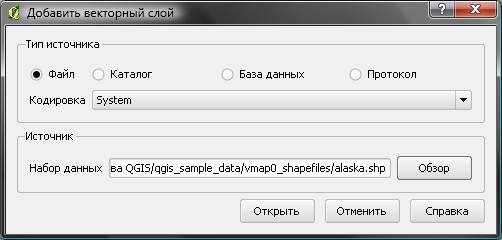
\includegraphics[clip=true, width=12cm]{addvectorlayerdialog}
   \caption{Диалог <<Добавить векторный слой>> \wincaption}\label{fig:addvectorlayer}
\end{figure}

\begin{figure}[ht]
   \centering
   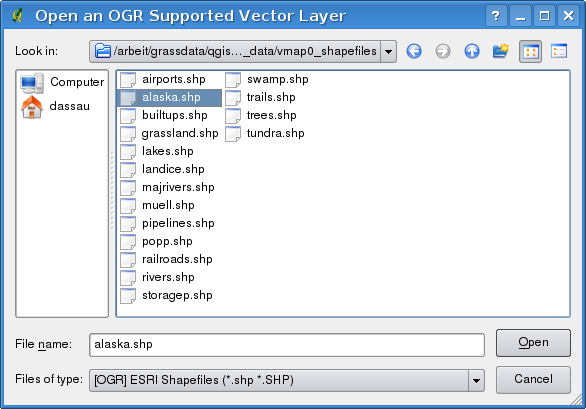
\includegraphics[clip=true, width=12cm]{shapefileopendialog}
   \caption{Диалог <<Открыть OGR-совместимый векторный слой>> \wincaption}\label{fig:openshapefile}
\end{figure}

\begin{figure}[ht]
   \centering
   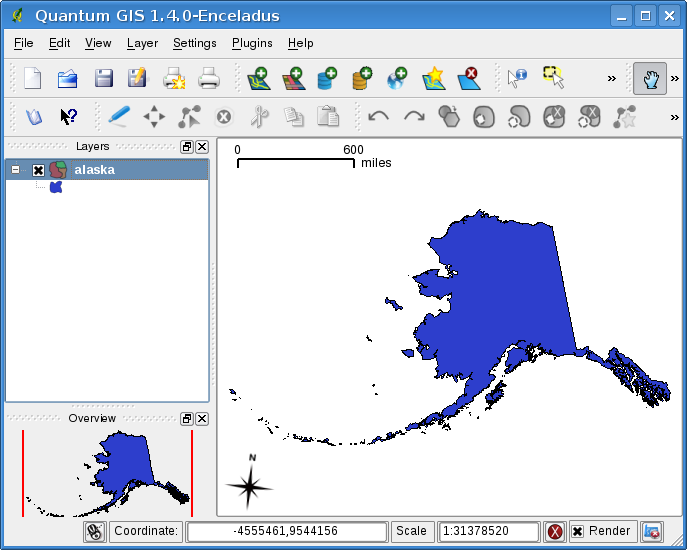
\includegraphics[clip=true, width=12cm]{shapefileloaded}
   \caption{\qg с загруженным shape-файлом Аляски \wincaption}\label{fig:loadedshapefile}
\end{figure}

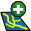
\includegraphics[width=0.7cm]{mActionAddNonDbLayer} Чтобы добавить shape-файл,
надо использовать кнопку \toolbtntwo{mActionAddNonDbLayer}{Добавить векторный слой}
\index{shape-файлы!загрузка} или сочетание клавиш \keystroke{Ctrl+Shift+V}.
Появится новое диалоговое окно (см. Рисунок~\ref{fig:addvectorlayer}).

В разделе <<Тип источника>> надо отметить \radiobuttonon{{}Файл}. Нажмите
кнопку \button{Обзор}. При этом появится стандартный диалог открытия файла
(см. Рисунок~\ref{fig:openshapefile}), который позволяет выбрать и добавить
нужный shape-файл или другой поддерживаемый источник данных. Выпадающее меню
фильтра типов файлов \selectstring{{}Тип файлов}\ldots позволяет фильтровать
файлы с форматами, поддерживаемыми библиотекой OGR.

Для выбранного shape-файла можно указать кодировку атрибутивных данных.

Выбор shape-файла из списка и нажатие кнопки \button{Открыть} загружает
файл в \qg. Рисунок~\ref{fig:loadedshapefile} демонстрирует \qg после
открытия файла \filename{alaska.shp}.


\begin{Tip}\caption{\textsc{Цвет слоя}}
Каждому вновь добавленному к карте слою присваивается случайный цвет.
Если было открыто несколько слоёв, каждому присваивается свой цвет,
отличный от других.
\end{Tip}

Для навигации по открытому shape-файлу можно воспользоваться инструментами
с панели навигации. Чтобы изменить символику слоя, следует открыть диалог
\dialog{Свойства слоя} двойным щелчком мыши на названии слоя или щёлкнув
правой кнопкой мыши на названии слоя в легенде и выбрав пункт
\dropmenuopt{Свойства} из всплывающего меню. Дополнительную информацию
о символике векторных слоёв можно найти в Разделе~\ref{sec:symbology}.

\begin{Tip}\caption{\textsc{Добавление слоя или проекта со внешнего носителя в OS\,X}}
В OS\,X подключённые внешние устройства не появляются после выбора <<Файл>> \arrow
<<Открыть проект>>. Мы работаем над разрешением этой проблемы в диалогах
открытия и сохранения в OS\,X. В качестве временного решения можно напечатать
<</Volumes>> в поле имени файла и нажать Ввод. После этого можно указать путь
ко внешним носителям и сетевым дискам.
\end{Tip}

\subsection{Улучшение производительности}

Для увеличения производительности при отрисовке shape-файла можно создать
пространственный индекс. Пространственный индекс \index{пространственный индекс!shape-файлы}
улучшает скорость отрисовки как при изменении масштаба, так и при
панорамировании (перемещении слоя в каком-либо направлении без изменения
масштаба). Файл пространственного индекса, используемого \qg, имеет
расширение \filename{.qix}.

Чтобы создать индекс, необходимо:

\begin{itemize}[label=--]
\item Открыть shape-файл.
\item Открыть диалог \dialog{Свойства соля} двойным щелчком по имени
shape-файла в легенде или правым щелчком по нему же и выбором
\dropmenuopt{Свойства} во всплывающем меню.
\item Во вкладке \tab{Общие} нажмите кнопку \button{Создать пространственный индекс}.
\end{itemize}

\subsection{Добавление слоя MapInfo к карте}
\index{векторные слои!MapInfo}

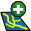
\includegraphics[width=0.7cm]{mActionAddNonDbLayer} Чтобы открыть слой
MapInfo, нажмите кнопку \toolbtntwo{mActionAddNonDbLayer}{Добавить
векторный слой} на панели инструментов или воспользуйтесь комбинацией
\keystroke{Ctrl+Shift+V}, измените \\
\selectstring{{}Тип файлов}{[OGR] MapInfo (*.mif*.tab *.MIF *.TAB)}
и выберите нужный файл.

\subsection{Добавление на карту покрытия ArcInfo}
\index{векторные слои!ArcInfo Binary Coverage}

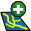
\includegraphics[width=0.7cm]{mActionAddNonDbLayer} Чтобы открыть покрытие ArcInfo
в двоичном формате, нажмите на кнопку
\toolbtntwo{mActionAddNonDbLayer}{Добавить векторный слой} на панели
инструментов или воспользуйтесь комбинацией клавиш \keystroke{Ctrl+Shift+V},
чтобы открыть диалог \dialog{Добавить векторный слой}. В качестве
<<Типа источника>> выберите \radiobuttonon{{}Каталог}. Выберите
\selectstring{{}Тип файлов}{Arc/Info Binary Coverage}. Укажите путь к каталогу
с файлами покрытия.

Аналогично добавляются векторные слои UK National Transfer Format и
TIGER Format Бюро переписи населения США (US Census Bureau).

\section{Слои PostGIS}
\index{векторные слои!PostGIS|see{PostGIS}}
\index{PostGIS!слои}
\label{label_postgis}

Слои PostGIS хранятся в базе данных PostgreSQL. Преимуществами PostGIS
являются пространственное индексирование и широкие возможности
фильтрации и построения запросов. При использовании PostGIS такие функции,
как выбор и идентификация, работают более точно, чем при использовании
OGR-совместимых слоёв.

Для использования слоёв PostGIS необходимо:\index{PostgreSQL!загрузка слоёв}

\begin{itemize}[label=--]
\item Задать настройки подключения \qg к базе данных PostgreSQL (если они
ещё не заданы).\index{PostgreSQL!подключение}
\item Соединиться с базой данных.
\item Выбрать нужный слой.
\item По желанию задать SQL-запрос \usertext{where}, определяющий конкретные
объекты из слоя, которые необходимо загрузить.
\item Добавить слой.
\end{itemize}

\subsection{Настройка подключения к базе данных PostGIS (PostgreSQL)}\index{PostgreSQL!подключение}\label{sec:postgis_stored}

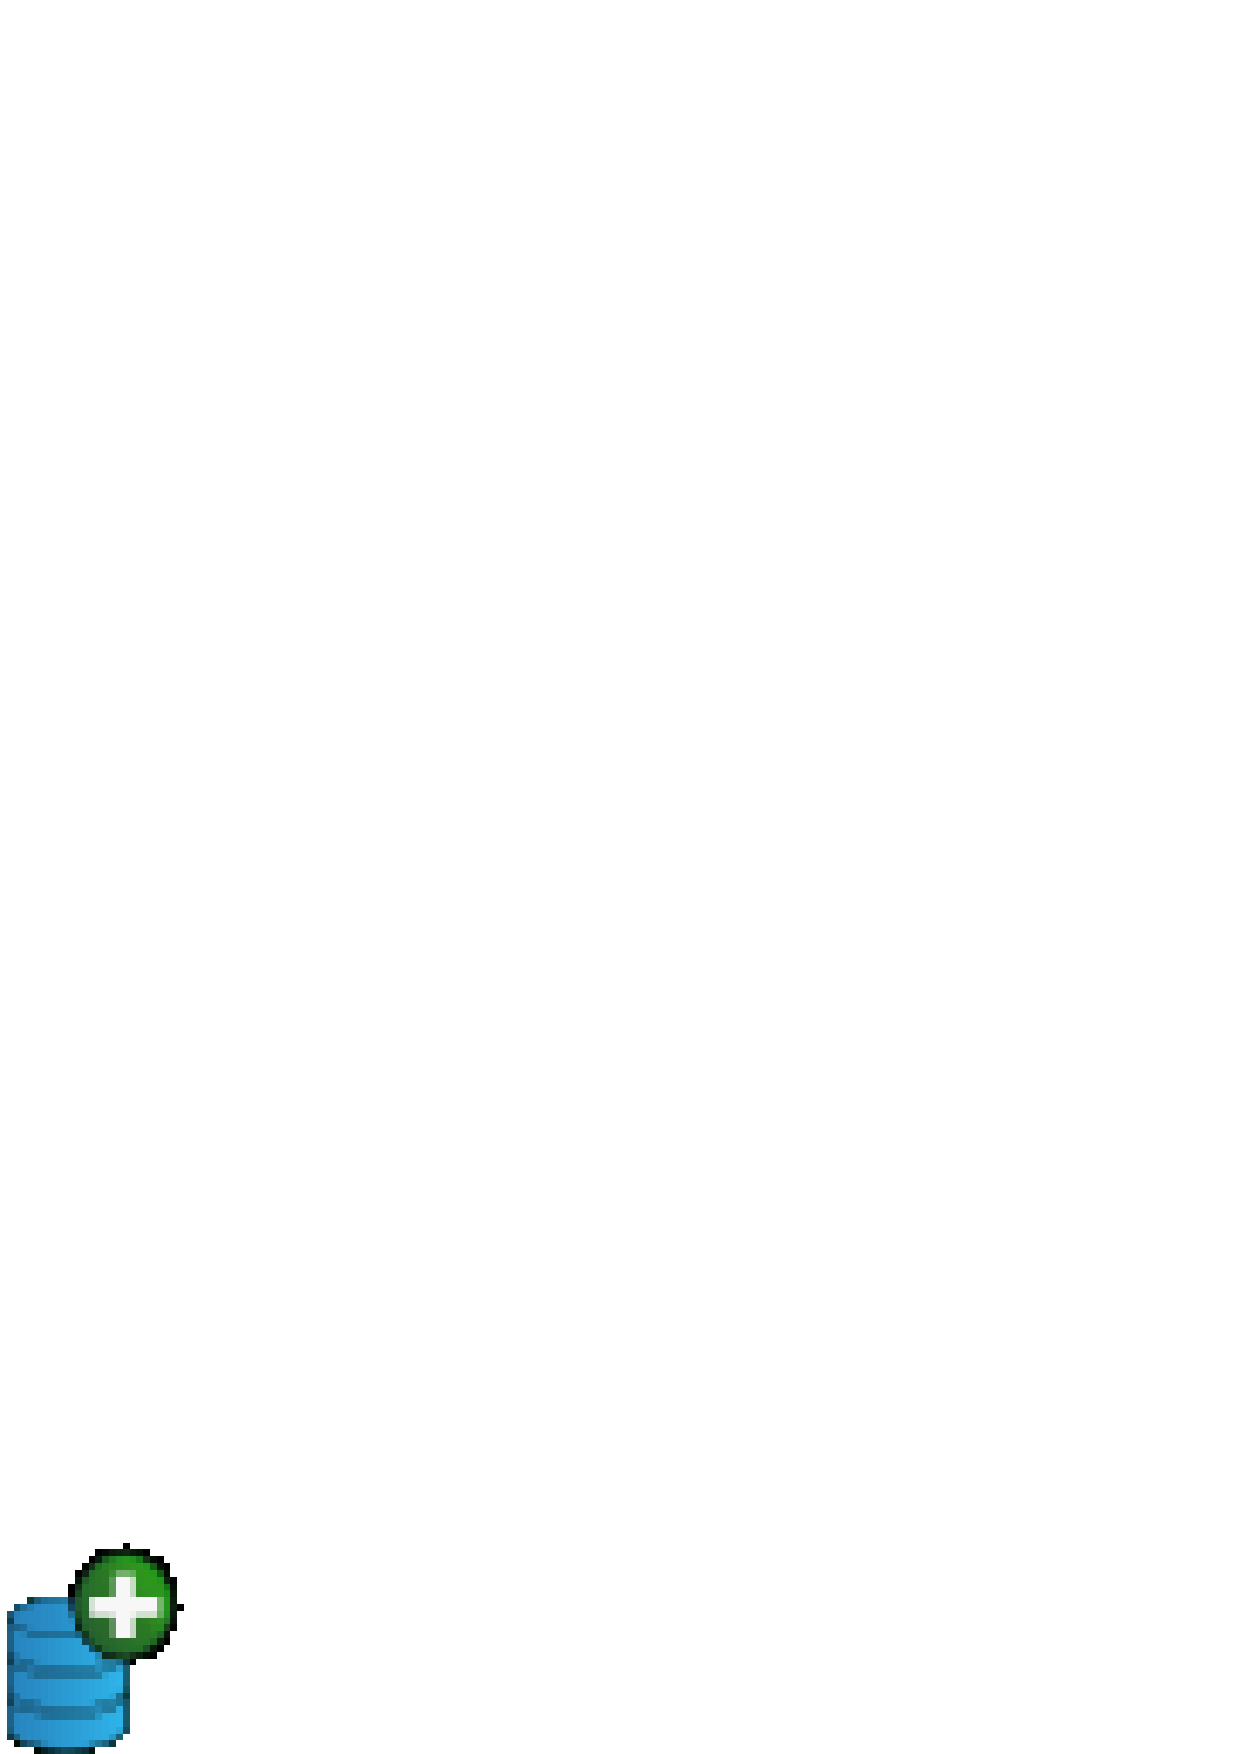
\includegraphics[width=0.7cm]{mActionAddLayer} При первом использовании
данных PostGIS необходимо настроить подключение к базе данных PostgreSQL,
содержащей нужную информацию. Нажмите на кнопку
\toolbtntwo{mActionAddLayer}{Добавить слой PostGIS} на панели инструментов
или выберите опцию \dropmenuopttwo{mActionAddLayer}{Добавить слой PostGIS\ldots}
из меню \mainmenuopt{Слой}, также можно воспользоваться комбинацией клавиш
\keystroke{Ctrl+Shift+D}. Ещё один вариант "--- открыть диалог
\dialog{Добавить векторный слой} и выбрать \radiobuttonon{{}База данных}.
Появится диалог \dialog{Добавить таблицы PostGIS}. Для получения доступа
к менеджеру соединений\index{PostgreSQL!менеджер соединений}, нажмите кнопку
\button{Создать}. \\
Появится диалог \dialog{Новое PostGIS соединение}. Параметры соединения
описаны в таблице~\ref{tab:postgis_connection_parms}.

\begin{table}[ht]\index{PostgreSQL!параметры подключения}
\centering
 \begin{tabular}{|l|p{5in}|}
\hline Имя & Имя для данного соединения. Может совпадать с именем\textsl{Базы данных}.
\\
\hline Узел \index{PostgreSQL!узел}
& Имя узла, на котором хранится база данных. Имя узла должно быть
допустимым"--- таким, какие используют для сетевого доступа или для пинга узла. Если база
данных находится на том же компьютере, что и \qg, просто введите здесь
<<localhost>>. \\
\hline База данных \index{PostgreSQL!база данных} & Имя базы данных. \\
\hline Порт \index{PostgreSQL!порт}& Номер порта, который <<слушает>>
сервер базы данных PostgreSQL. По умолчанию используется порт 5432.\\
\hline SSL-режим \index{PostgreSQL!режим SSL}& Настройка SSL-режима работы
с сервером. Можно выбрать:
\begin {itemize}
\item запретить: использовать только не зашифрованное SSL-соединение;
\item разрешить: будет произведена попытка установки не SSL-соединения,
если она не удастся, будет использовано SSL-соединение;
\item предпочитать (по умолчанию): будет произведена попытка установки
SSL-соединения, если она не удастся, будет использовано не SSL-соединение;
\item требовать: использовать только SSL-соединение.
\end {itemize}
Следует отметить, что значительного прироста скорости рендеринга слоя PostGIS
можно достигнуть путём отключения SSL в менеджере соединений. \\
\hline Пользователь \index{PostgreSQL!пользователь}& Имя пользователя, которое
используется для доступа к базе данных. \\
\hline Пароль \index{PostgreSQL!пароль}& Пароль, используемый вместе с
\textsl{именем пользователя} для подключения к базе данных.\\
\hline
\end{tabular}
\caption{Параметры подключения PostGIS}\label{tab:postgis_connection_parms}\medskip
\end{table}

Есть возможность выбрать дополнительные параметры:

\begin{itemize}[label=--]
\item \checkbox{Сохранить пользователя}
\item \checkbox{Сохранить пароль}
\item \checkbox{Искать только в таблице <<geometry\_columns>>}
\item \checkbox{Искать только в схеме <<public>>}
\item \checkbox{Использовать расчётные метаданные таблицы}
\end{itemize}

Когда параметры установлены, можно проверить соединение путём нажатия
на кнопку \button{Проверить соединение} \index{PostgreSQL!соединение!проверка}.

\begin{Tip}\caption{\textsc{\qg Пользовательские настройки и безопасность}}
\index{настроки}\index{безопасность}
В зависимости от используемой операционной системы \qg хранит
пользовательские настройки: в <<домашнем>> каталоге на \nix системах
\filename{.\qg/}; в реестре, если используется \win. В зависимости
от используемой операционной системы и настроек компьютера, хранение пароля
в настройках \qg может создавать угрозу безопасности.
\end{Tip}

\subsection{Добавление слоя PostGIS к карте}\index{PostgreSQL!загрузка слоёв}

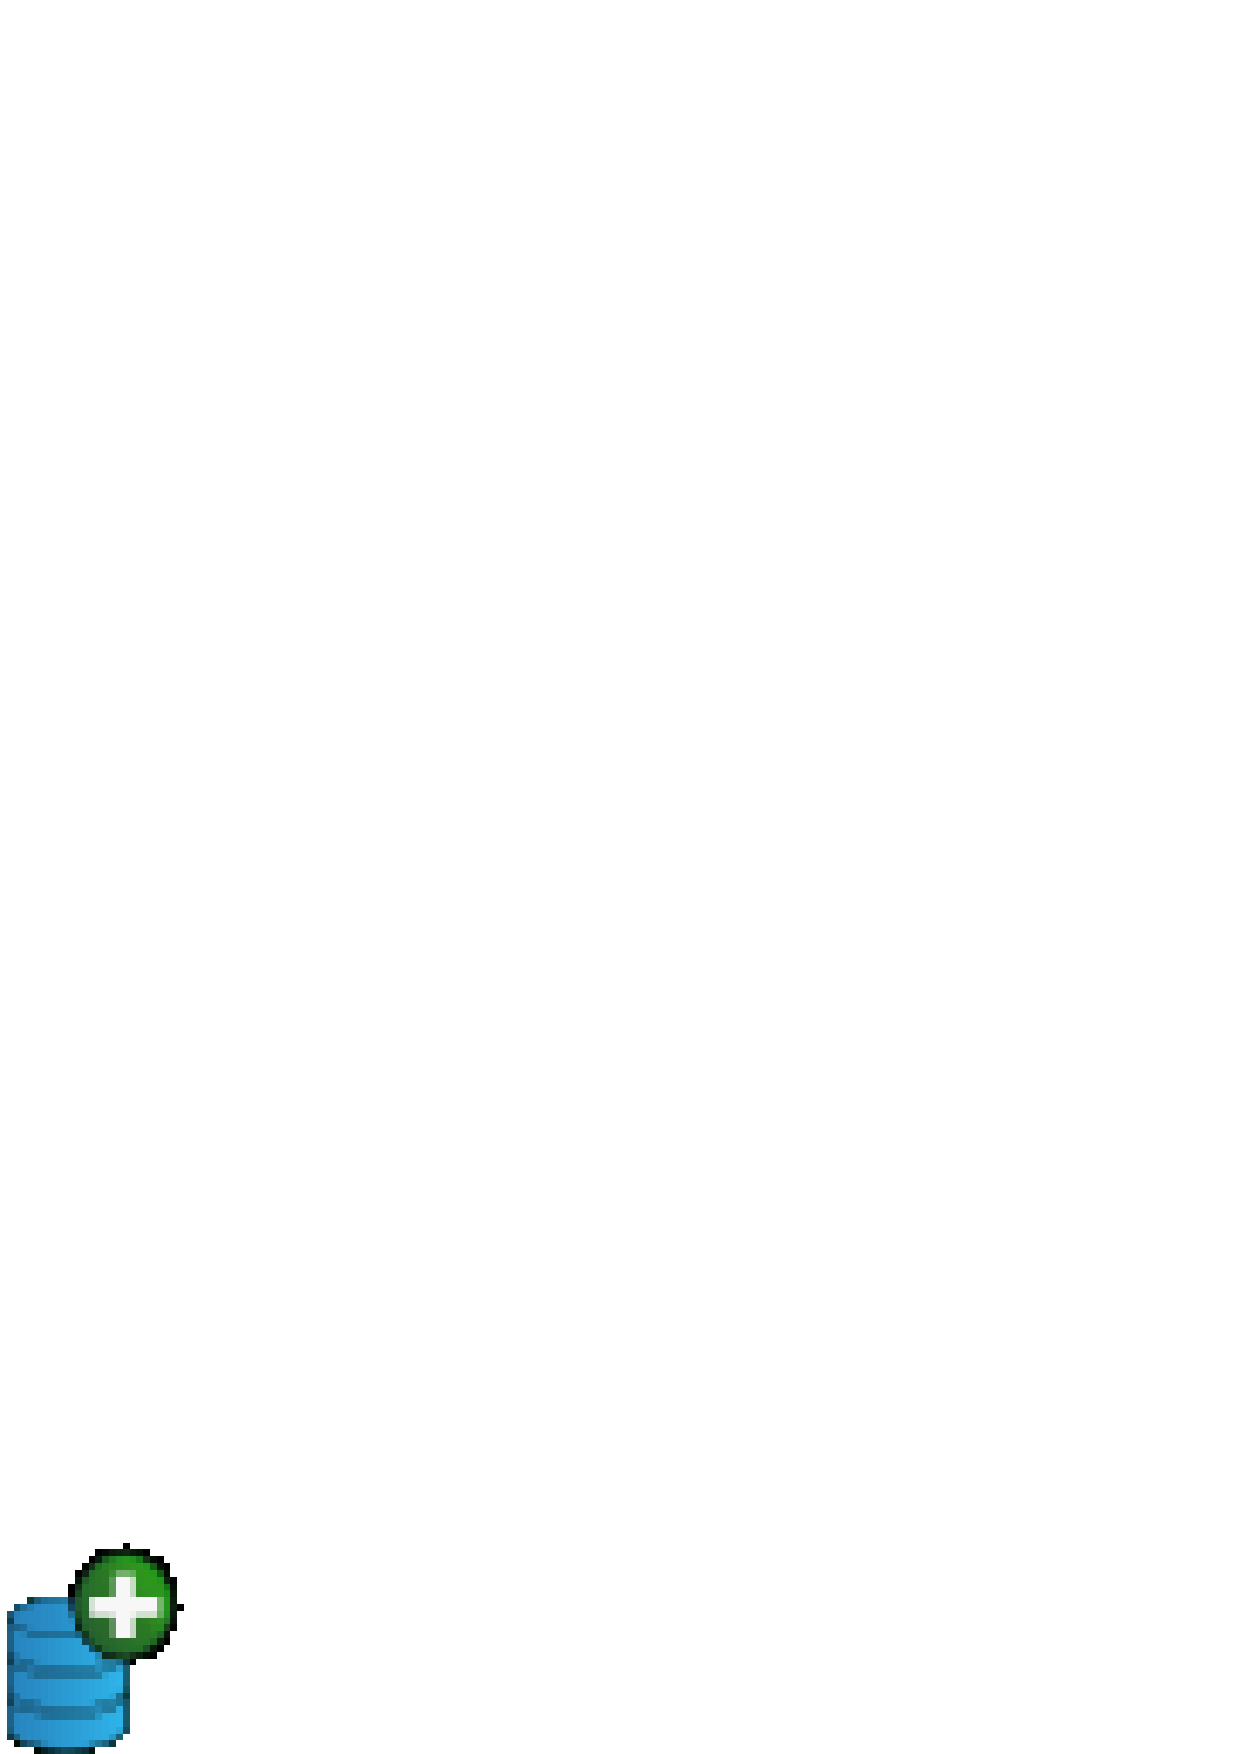
\includegraphics[width=0.7cm]{mActionAddLayer} Когда создано одно или
более соединение, можно добавлять слои из PostgreSQL. Естественно, в базе
данных PostgreSQL должна содержаться
информация. См.~Раздел~\ref{sec:loading_postgis_data}, в котором
обсуждается импорт данных в базу данных.

Для открытия слоя PostGIS проделайте следующие шаги:

\begin{itemize}[label=--]
\item Если диалог \dialog{Add PostGIS Table(s)} ещё не открыт, нажмите
кнопку \toolbtntwo{mActionAddLayer}{Добавить слой PostGIS} на панели
инструментов.
\item Выберите соединение из выпадающего списка и нажмите кнопку
\button{Подключиться}.
\item Найдите слой, который желаете добавить в список доступных слоёв.
\item Щёлкните по нему, чтобы выбрать. Можно выбрать несколько слоёв,
если нажать и удерживать клавишу \keystroke{Shift}. В
Разделе~\ref{sec:query_builder} можно найти информацию об использовании
<<Конструктора запросов>> при работе с PostgreSQL.
\item Нажмите кнопку \button{Добавить}, чтобы добавить слой к карте.
\end{itemize}

\begin{Tip}\caption{\textsc{Слои PostGIS}}
Обычно слои PostGIS определяются наличием записей в таблице
geometry\_columns. Начиная с версии \OLD\, % should be 0.9.0
\qg может загружать слои, которые не имеют записей в таблице
geometry\_columns. Это касается таблиц и <<представлений>>.
Задание пространственных представлений "--- мощное средство визуализации данных.
В руководстве пользователя PostgreSQL можно найти дополнительную информацию
по созданию представлений.
\end{Tip}

\subsection{Некоторые особенности работы со слоями PostgreSQL}
\label{sec:postgis_details}
\index{PostgreSQL!особенности}

Этот раздел содержит некоторые подробности доступа к слоям PostgreSQL в \qg.
Обычно \qg обеспечивает доступ к списку таблиц базы данных, которые можно
добавить к карте и открывает их по запросу. Однако, если возникают трудности
с открытием таблиц PostgreSQL, следующая информация может помочь
понять сообщения \qg и подсказать способы изменения способа определения
таблицы или представления PostgreSQL.

\qg требует наличия колонки в слое PostgreSQL, которая бы служила уникальным
идентификатором (ключом) слоя. Для таблиц это обычно означает, что они должны
иметь первичный ключ, или колонку с уникальными значениями строк в ней.
В \qg эта колонка должна содержать значения типа int4 (целое число размером
4 байта). Альтернативный способ "--- использование колонки <<ctid>> в качестве
первичного ключа. Если в таблице отсутствуют колонки, указанные выше, то
вместо них будет использоваться колонка <<oid>>. Индексирование колонок позволит
повысить производительность (заметьте, что первичные ключи в PostgreSQL
индексируются автоматически).

Если слой PostgreSQL является представлением, к нему предъявляются те же
требования, что были описаны выше, но представления не имеют первичных
ключей или колонок с уникальными значениями. В этом случае \qg попытается
самостоятельно найти колонку в представлении, являющуюся производной от
колонки, удовлетворяющей необходимым условиям. Это достигается посредством
разбора SQL-опеределения представления. Однако, есть элементы SQL,
игнорируемые \qg, например, использование псевдонимов таблиц и колонок,
создаваемых SQL-запросами.

Если невозможно найти подходящую колонку, \qg не откроет слой. В таком
случае следует изменить представление таким образом, чтобы оно содержало
требуемую колонку (тип int4 и либо являющуюся первичным ключом, либо
содержащую уникальные значения, желательно, индексированную).

%%FIXME: Add missing information
%% When dealing with views, \qg parses the view definition and

\subsection{Импорт данных в PostgreSQL}\label{sec:loading_postgis_data}
\index{PostGIS!SPIT!импорт данных}

\minisec{shp2pgsql}
Существует несколько способов импорта данных в базу данных PostgreSQL. PostGIS
поставляется с утилитой \filename{shp2pgsql}, которую можно использовать для
импорта shape-файлов в базу данных PostGIS. Например для импорта shape-файла
\filename{lakes.shp} в базу данных PostgreSQL, называющуюся
\usertext{gis\_data}, воспользуйтесь следующей командой:

\begin{verbatim}
  shp2pgsql -s 2964 lakes.shp lakes_new | psql gis_data
\end{verbatim}

При этом будет создан новый слой под названием \usertext{lakes\_new} в
базе данных \usertext{gis\_data}. Новый слой будет иметь идентификатор
системы координат (SRID) 2964. более подробную информацию о системах координат
и проекциях можно найти в Разделе~\ref{label_projections}
\begin{Tip}
\caption{\textsc{Экспорт наборов данных из PostGIS}\index{PostGIS!экспорт}}
Наряду с инструментом для импорта \filename{shp2pgsql} существует инструмент
для экспорта наборов данных PostGIS в shape-файл: \filename{pgsql2shp}.
Он также входит в поставку PostGIS.
\end{Tip}

\minisec{Модуль SPIT}

\includegraphics[width=0.7cm]{spiticon} \qg включает в себя модуль
SPIT (Shapefile to PostGIS Import Tool "--- инструмент импорта shape-файлов
в PostGIS)\index{PostGIS!SPIT}. SPIT способен осуществлять одновременный
импорт нескольких shape-файлов и поддерживает схемы баз данных. Для
использования SPIT откройте <<Менеджер управления модулями>> \qg в меню
\mainmenuopt{Модули} и выберите пункт <<Управление модулями>>, поставьте
галочку напротив \checkbox{SPIT} и нажмите кнопку \button{OK}. Иконка
модуля SPIT появится на панели инструментов\index{PostGIS!SPIT!загрузка}.

Для импорта shape-файла нажмите на иконку \toolbtntwo{spiticon}{SPIT}
на панели инструментов. \\
Откроется диалог \dialog{SPIT "--- инструмент импорта shape-файлов в PostGIS}.
Выберите базу данных PostGIS, с которой необходимо установить соединение, и
нажмите кнопку \button{Подключиться}. Теперь можно добавить файлы в
очередь, нажимая кнопку \button{Добавить}. Для запуска обработки файлов
нажмите кнопку \button{OK}. Прогресс импорта, так же, как и любые ошибки
или предупреждения, будет показан после обработки каждого из shape-файлов.

\begin{Tip}\caption{\textsc{Импорт shape-файлов, содержащих
слова, зарезервированные PostgreSQL}}\index{PostGIS!SPIT!зарезервированные слова}
Если shape-файл, добавленный в очередь, содержит имена полей, зарезервированные
базой данных PostgreSQL, появится диалог, сообщающий статус каждого поля.
Можно изменить имена этих (и других) полей\index{PostGIS!SPIT!редактирование имен полей}
перед импортом. Попытки импорта shape-файла с именами полей, зарезервированными
PostgreSQL, обречены на провал.
\end{Tip}

\minisec{ogr2ogr}
Кроме \filename{shp2pgsql} и \filename{SPIT} есть ещё один инструмент
импорта пространственной информации в PostGIS "--- \filename{ogr2ogr}, "---
который является частью установки GDAL. Для импорта shape-файла в PostGIS
проделайте следующее (в \nix):
\begin{verbatim}
  ogr2ogr -f "PostgreSQL" PG:"dbname=postgis host=myhost.de user=postgres \
  password=topsecret" alaska.shp
\end{verbatim}

Эта команда импортирует файл \filename{alaska.shp} в базу данных PostGIS
\usertext{postgis} на сервере \server{myhost.de}, используя в качестве
имени пользователя базы данных \usertext{postgres} с паролем \usertext{topsecret}.

Заметьте, что для работы с PostGIS в OGR должна быть включена поддержка
PostgreSQL. Проверить её наличие можно с помощью команды (в \nix)
\begin{verbatim}
ogrinfo --formats | grep -i post
\end{verbatim}

Те, кто предпочитают использовать команду PostgreSQL \filename{COPY}
вместо метода \filename{INSERT INTO}, используемого по умолчанию, могут
экспортировать следующие переменные среды (доступно, по крайней мере, для
\nix и \\ \osx):
\begin{verbatim}
  export PG_USE_COPY=YES
\end{verbatim}

\filename{ogr2ogr} не создаёт пространственный индекс, как это делает
\filename{shp2pgsl}. Его необходимо создать вручную, используя SQL-команду
\filename{CREATE INDEX} после экспорта (смотри описание в следующем
Разделе~\ref{label_improve}).

\subsection{Повышение производительности} \label{label_improve}

Получение данных, находящихся в базе данных PostgreSQL, может серьёзно
снижать производительность, особенно при работе через сеть. Производительность
при отрисовке можно улучшить путём создания пространственного индекса для
каждого слоя базы данных PostgreSQL \index{PostGIS!пространственный индекс}.
PostGIS поддерживает создание \index{PostGIS!пространственный индекс!GiST} GiST-индекса
(Generalized Search Tree) для ускорения пространственного поиска данных.

Ниже представлен порядок создания GiST\footnote{Информация о GiST-индексе
взята из документации к PostGIS, доступной на
\url{http://postgis.refractions.net}}-индекса:

\begin{verbatim}
    CREATE INDEX [indexname] ON [tablename]
      USING GIST ( [geometryfield] GIST_GEOMETRY_OPS );
\end{verbatim}

Заметьте, что для больших таблиц создание индекса может занять
продолжительное время. После создания индекса следует произвести
\usertext{VACUUM ANALYZE}. Дополнительную информацию можно найти в
документации к PostGIS \cite{PostGISweb}.

Приведём пример создания GiST-индекса (\nix):
\begin{verbatim}
gsherman@madison:~/current$ psql gis_data
Welcome to psql 8.3.0, the PostgreSQL interactive terminal.

Type:  \copyright for distribution terms
        \h for help with SQL commands
        \? for help with psql commands
        \g or terminate with semicolon to execute query
        \q to quit

gis_data=# CREATE INDEX sidx_alaska_lakes ON alaska_lakes
gis_data-# USING GIST (the_geom GIST_GEOMETRY_OPS);
CREATE INDEX
gis_data=# VACUUM ANALYZE alaska_lakes;
VACUUM
gis_data=# \q
gsherman@madison:~/current$
\end{verbatim}

\subsection{Векторные слои, пересекающие долготу 180$^\circ$}
\index{векторные слои!пересечение линии дат}

Многие ГИС испытывают трудности при работе с векторными картами в системе
координат широта/долгота (lat/lon), пересекающими долготу \degrees{180}.
При открытии таких карт в \qg можно наблюдать две разнесённые на большое
удаление друг от друга части территории/акватории, которые на самом деле
представляют собой единое целое. На Рисунке~\ref{fig:vector_not_wrapping}
едва заметные точки в левой части карты (архипелаг Чатем), должны
находиться внутри сетки, справа от главных островов (Северного и Южного)
Новой Зеландии.

\begin{figure}[ht]
   \centering
   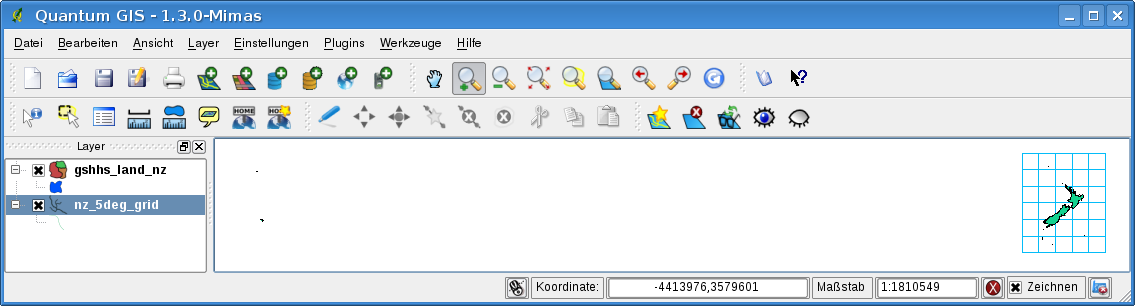
\includegraphics[clip=true, width=\textwidth]{vectorNotWrapping}
      \caption{Карта в системе координат широта/долгота, пересекающая долготу \degrees{180} \wincaption}
   \label{fig:vector_not_wrapping}
\end{figure}

В качестве одного из вариантов решения проблемы можно предложить трансформацию
значений координат долготы при помощи PostGIS и функции
\textbf{ST\textunderscore Shift\textunderscore Longitude}
\footnote{\url{http://postgis.refractions.net/documentation/manual-1.4/ST\_Shift\_Longitude.html}}.
Эта функция проверяет каждую точку (или узел) каждого объекта слоя, и,
если координаты долготы < \degrees{0}, добавляет \degrees{360} к значению.
На результирующей карте долгота объектов будет лежать в пределах
\degrees{0} -- \degrees{360} а сама карта будет отцентрирована по
\degrees{180} долготы.

\begin{figure}[ht]
   \centering
   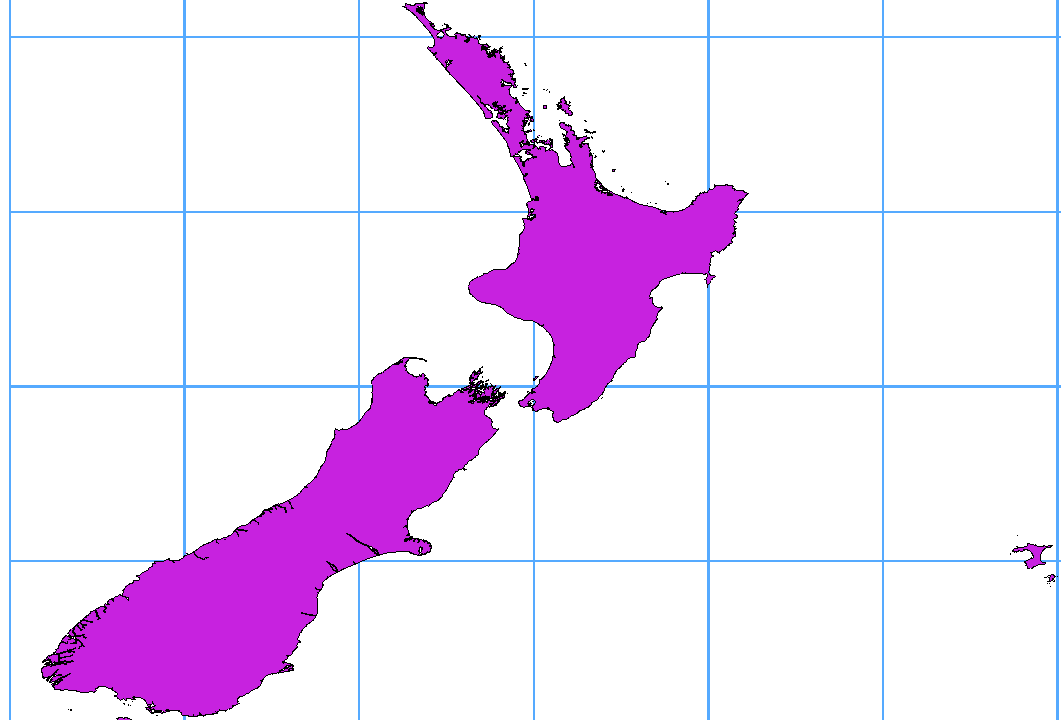
\includegraphics[clip=true, width=9cm]{vectorWrapping}
   \caption{Карта, пересекающая долготу \degrees{180}, после применения функции ST\textunderscore Shift\textunderscore Longitude \wincaption}
\label{fig:vector_wrapping}
\end{figure}

\minisec{Использование}

\begin{itemize}[label=--]
\item Импортируем данные в PostGIS (\ref{sec:loading_postgis_data}) при помощи
модулей <<PostGIS Manager>> или <<SPIT>>
\item Используя командную строку PostGIS, выполните следующую команду
(в этом примере <<TABLE>> "--- имя вашей таблицы PostGIS): \\
\texttt{gis\_data=\# update TABLE set the\_geom=ST\_shift\_longitude(the\_geom);}
\item Если операция прошла успешно, появится подтверждение о количестве
объектов, информация о которых обновлена, после этого будет возможно добавить
объекты на карту и увидеть изменения (см. Рисунок~\ref{fig:vector_wrapping})
\end{itemize}

\section{Слои SpatiaLite}
\index{слои SpatiaLite!свойства}
\index{векторные слои!SpatlaLite|see{SpatiaLite}}
\index{SpatiaLite!слои}
\label{label_spatialite}

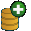
\includegraphics[width=0.7cm]{mActionAddSpatiaLiteLayer}
При первой загрузке слоёв из базы данных SpatiaLite воспользуйтесь кнопкой \\
\toolbtntwo{mActionAddSpatiaLiteLayer}{Добавить слой SpatiaLite}
на панели инструментов или пунктом
\dropmenuopttwo{mActionAddSpatiaLiteLayer}{Добавить слой SpatiaLite\ldots}
меню \mainmenuopt{Слой}, либо комбинацией клавиш \keystroke{Сtrl+Shift+L}.
Появится окно, позволяющее соединиться с базой данных SpatiaLite,
которая уже была подключена к \qg ранее (её можно выбрать в выпадающем
меню), или же создать новое подключение. Для создания нового подключения
нажмите на кнопку \button{Создать} и используйте менеджер файлов, чтобы
указать путь к нужной базе данных (файлу с расширением \filename{.sqlite }).

\section{Свойства векторного слоя}\label{sec:vectorprops}
\index{векторные слои!свойства}

Диалог \dialog{Свойства слоя} для векторного слоя предоставляет информацию
о слое, настройках символики и подписей. Если ваш векторный слой был загружен
из хранилища PostgreSQL/PostGIS, вы также можете изменить лежащий в его
основе SQL, вызвав диалог \dialog{Построитель запросов} во вкладке \tab{Общие}.
Чтобы вызвать диалог \dialog{Свойства слоя}, дважды щелкните мышью на слое в
легенде или сделайте щелчок правой кнопкой мышки на нем и выберите
\dropmenuopt{Свойства} в контекстном меню.

\begin{figure}[ht]
   \centering
   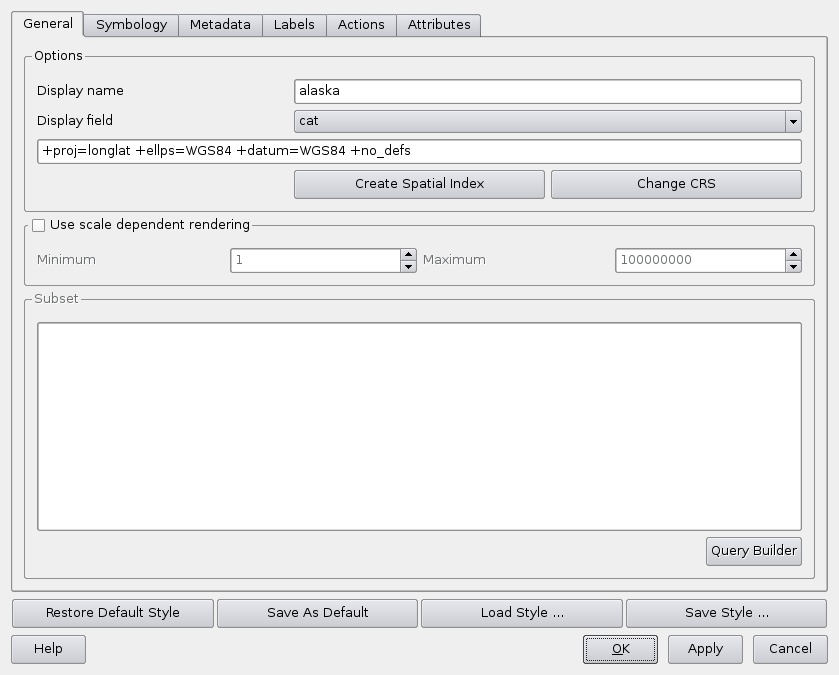
\includegraphics[clip=true, width=12cm]{vectorLayerSymbology}
   \caption{Свойства векторного слоя \wincaption}\label{fig:vector_symbology}
 \end{figure}

\subsection{Символика}\label{sec:symbology}
\index{векторные слои!символика}

\qg поддерживает целый ряд представлений символики для контроля за
 отображением векторных объектов. На данный момент доступны следующие
типы:

\begin{description}
    \item[Обычный знак] "--- единый стиль применяется к каждому
    объекту слоя.\index{векторные слои!легенда!обычный знак}
    \item[Градуированный знак] "--- объекты слоя
    отображаются различными символами, которые определяются значениями
    определенного поля.\index{векторные слои!легенда!градуированный знак}
    \item[Непрерывный цвет] "--- объекты слоя отображаются цветами из
    диапазона, который определяется числовыми значениями указанного поля.\index{векторные слои!легенда!непрерывный цвет}
    \item[Уникальное значение] "--- объекты классифицируются уникальными
    значениями указанного поля, где каждому значению соответствует
    различный символ.\index{векторные слои!легенда!уникальное значение}
\end{description}

Для того, чтобы изменить символику слоя, просто сделайте двойной щелчок
мышью на его записи в легенде и откроется диалог \dialog{Свойства слоя}.\index{симовлика!изменение}

\begin{figure}[ht]
\centering
   \subfloat[Обычный знак] {\label{subfig:single_symbol}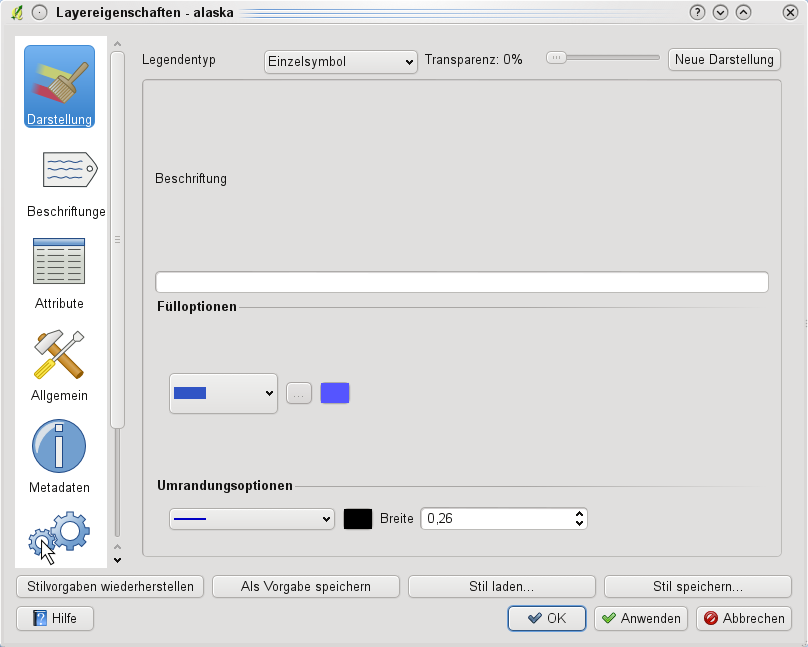
\includegraphics[clip=true, width=0.4\textwidth]{vectorClassifySingle}}
   \hspace{1cm}
   \subfloat[Градуированный знак] {\label{subfig:graduated_symbol}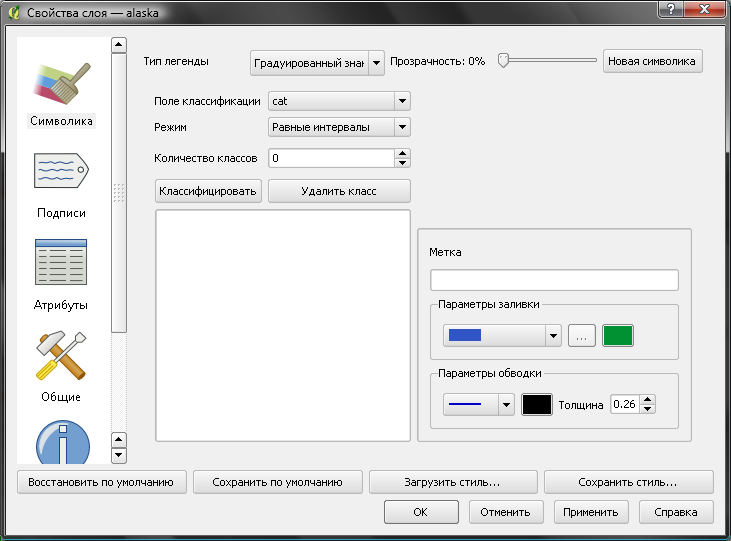
\includegraphics[clip=true, width=0.4\textwidth]{vectorClassifyGraduated}}
   \hspace{1cm}
   \subfloat[Непрерывный цвет] {\label{subfig:cont_color}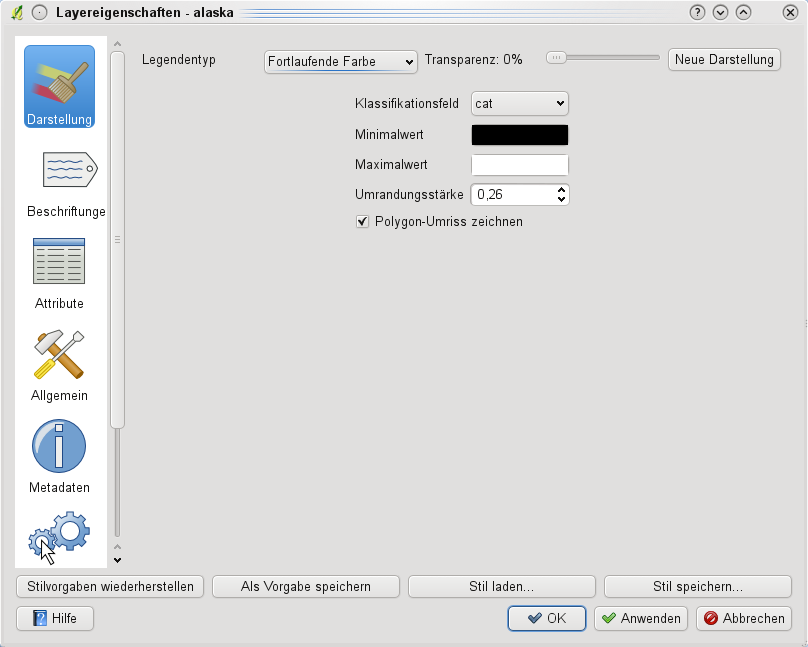
\includegraphics[clip=true, width=0.4\textwidth]{vectorClassifyContinous}}
   \hspace{1cm}
   \subfloat[Уникальное значение] {\label{subfig:unique_val}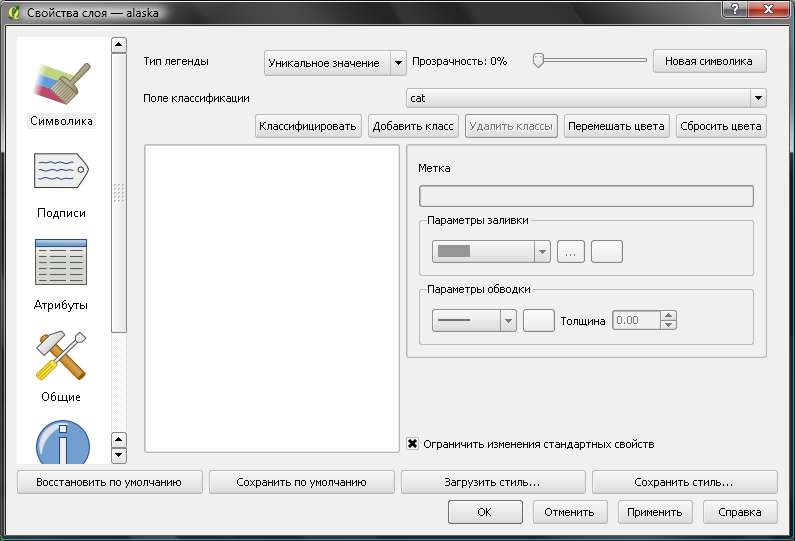
\includegraphics[clip=true, width=0.4\textwidth]{vectorClassifyUnique}}
\caption{Опции символики \wincaption}
\end{figure}

% FIXME: outdated
% Since \usertext{version v0.9} there is a function to use image files stored on
% your computer as fill pattern for vector layers.

\minisec{Параметры стиля} \label{sec:style_options} \index{векторные слои!стили}
В диалоге вы можете задать стиль векторного слоя. В зависимости от
выбранного варианта легенды, имеется возможность также классифицировать
объекты карты.

Следующие параметры стиля задаются для всех представлений символики:
\begin{description}
\item[Параметры заливки]
\begin{description}
 \item[Стиль заливки] "--- кроме имеющихся типов заливки, вы
 можете выбрать \selectstring{{}Стиль заливки}{? Текстура} и щелкнуть на
 кнопке \browsebutton для выбора вашего собственного файла текстуры. На
 данный момент поддерживаются форматы \filename{*.jpeg, *.xpm и *.png}.
 \item[Цвет заливки] "--- цвет заливки объектов.
\end{description}
\item[Параметры обводки]
\begin{description}
 \item[Стиль контура] "--- стиль контура объекта. Вы можете
 также установить значение <<Нет>> для этой опции.
 \item[Цвет контура] "--- цвет контура вашего объекта.
 \item[Толщина] "--- толщина ваших объектов.
\end{description}
\end{description}

Однажды определив стиль своего слоя, вы можете сохранить этот стиль в
отдельном файле (с расширением \filename{*.qml}). Чтобы сделать это,
используйте кнопку \button{Сохранить стиль\ldots}. Нет необходимости
напоминать, что нажатие кнопки \button{Загрузить стиль\ldots} приведет к
загрузке вашего сохраненного файла стиля слоя.

Если вы хотите всегда использовать конкретный стиль для всех загружающихся
слоёв, используйте кнопку \button{Сохранить как значение по умолчанию},
чтобы сделать ваш стиль стилем по умолчанию. Также, если внесенные изменения
вас не удовлетворяют, используйте кнопку \button{Восстановить по умолчанию},
чтобы возвратиться к вашему стилю по умолчанию.

\minisec{Прозрачность вектора} \label{sec:vect_transparency}
\index{векторные слои!прозрачность}

\qg позволяет устанавливать прозрачность для каждого векторного слоя. Это
можно сделать при помощи ползунка \slider{Прозрачность} во вкладке \tab{Символика}
(см. Рисунок~\ref{subfig:single_symbol}). Это бывает полезно при наложении
нескольких векторных слоёв.

\subsection{Новая символика}

Начиная с версии \qg 1.4.0, параллельно с символикой, описанной выше, была
внедрена новая символика. Символика нового поколения содержит множество
улучшений и новых функций и заместит текущую (<<старую>>) символику в одной из
предстоящих версий. Для перехода на новую символику в текущей версии вы
должны щелкнуть на кнопке \button{Новая символика} на вкладке \tab{Символика}
диалога \dialog{Свойства слоя}. Вы также можете указать, чтобы новая символика
использовалась по умолчанию, установив флажок \\
\checkbox{Использовать новую реализацию отрисовки условных знаков} во вкладке
\tab{Отрисовка} в меню \mainmenuopt{Установки} \arrow \dropmenuopt{Пераметры}.

\minisec{Понимание новой символики}

Существует три типа символов: маркерные символы (для точек), линейные символы
и символы заполнения (для полигонов). Символы могут состоять из одного или
нескольких символьных слоёв. Можно установить цвет символа, и этот цвет
установится для всех символьных слоёв. Цвет некоторых слоёв может быть
заблокированным "--- для этих слоёв цвет изменять запрещается. Это полезно,
когда вы устанавливаете цвет для символа, состоящего из нескольких слоев.
Подобным образом можно устанавливать ширину линейных символов, а также
размер и угол маркерных символов.

\minisec{Доступные типы символов слоя}

\begin{itemize}[label=--]
\item \textbf{Простой маркер}: отрисовка с использованием одного из
предустановленных маркеров.
\item \textbf{Простая линия}: обычная отрисовка линии (с указанными
шириной, цветом и стилем).
\item \textbf{Простая заливка}: обычная отрисовка полигона (с определенным
цветом заливки, шаблоном заливки и контуром).
\item \textbf{SVG маркер}: отрисовка с использованием SVG изображения.
\item \textbf{Линия маркеров}: отрисовка линии повторением маркерного символа.
\end{itemize}

\minisec{Цветовые шкалы}

Цветовые шкалы применяются для задания диапазона цветов,
использующихся при отрисовке. Цвет символа будет установлен
из цветовой шкалы.

Существует три типа цветовых шкал:

\begin{itemize}[label=--]
\item \textbf{Градиент}: линейный градиент одного цвета к другому.
\item \textbf{Случайная}: случайным образом сгенерированные цвета из
указанной области цветового пространства.
\item \textbf{ColorBrewer}: создает цветовую область из цветовой схемы и
определенного количества цветовых классов.
\end{itemize}

Цветовые шкалы можно задать в диалоге \dialog{Управление стилями}
(см. Раздел~\ref{subsec:stylemanager}), выбрав \\
\selectstring{{}Тип условного знака}{Градиент} в качестве типа стиля
 элемента из выпадающего списка, щелкнув на кнопке \button{Добавить элемент}
 и затем выбрав тип цветовой шкалы.

\minisec{Стили}

Группы стилей "--- это множество различных символов и цветовых шкал. Вы
можете определить предпочтительные для вас или часто используемые символы,
и в дальнейшем использовать их без необходимости создавать каждый раз заново.
Элементы стиля (символы и цветовые шкалы) всегда имеют имена, по которым
их можно получить из стиля. В \qg имеется один (изменяемый) стиль по
умолчанию, а пользователь может добавлять дополнительные стили.

\minisec{Отрисовка (тип легенды)}

Рендер осуществляет прорисовку элемента соответствующим символом.
Существует три типа легенды: обычный знак, уникальные значения (категории)
и градуированный знак. Отрисовка непрерывным цветом не выделяется в отдельный
тип, т.\,к. по сути является частным случаем отрисовки градациями.
Отрисовку категориями и градациями можно создать, указав символ
и цветовую шкалу "--- они установят цвета для символов соответствующим
образом.

\subsection{Использование символики нового поколения}

Сначала вы должны сделать символику нового поколения доступной, нажав
кнопку \button{Новая символика} во вкладке \tab{Символика} диалога
\dialog{Свойства слоя}. Новый диалог позволяет выбрать один из
трёх типов легенды: обычный знак, уникальные значения (категории)
и градуированный знак. В зависимости от выбранного типа легенды, вкладка
символики предоставляет различные настройки и опции, которые будут описаны
в следующих разделах.

\minisec{Отрисовка обычным знаком}

Тип легенды <<обычный знак>> используется для отрисовки всех элементов слоя с
использованием одного, определенного пользователем, символа. Свойства, которые
можно задать во вкладке символики, частично зависят от типа слоя, но у всех
типов имеется следующая общая структура. В левой верхней части вкладки
показана уменьшенная копия текущего символа отрисовки. В нижней части
вкладки приведен список ранее установленных символов текущего стиля, начать
использование которых можно, выбрав их из списка. Текущий символ можно
изменить, воспользовавшись кнопкой \button{Свойства}, нажатие которой
открывает диалог \dialog{Свойства символов}, или кнопкой \button{Задать цвет},
нажатие которой открывает стандартный диалог \dialog{Цвет}. После внесения
любых необходимых изменений, символ можно добавить к списку текущих символов
стиля (с помощью кнопки \button{Добавить к стилю}), и потом им можно будет
легко пользоваться в будущем.

\begin{figure}[ht]
\centering
   \subfloat[Свойства точечного символа] {\label{subfig:singleNG1}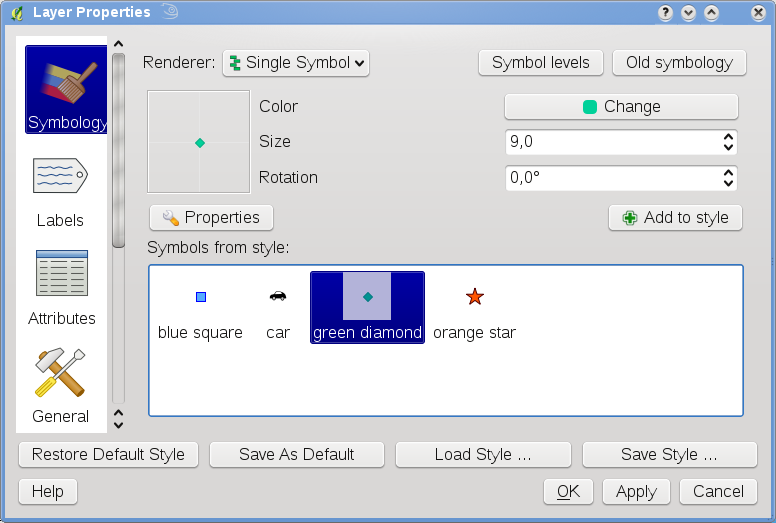
\includegraphics[clip=true, width=0.3\textwidth]{singlesymbol_ng_point}}
   \hspace{1cm}
   \subfloat[Свойства линейного символа] {\label{subfig:singleNG2}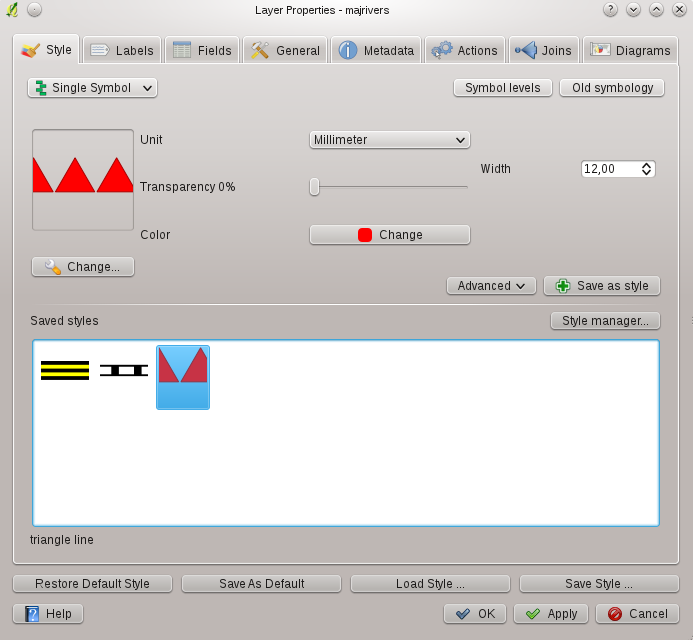
\includegraphics[clip=true, width=0.3\textwidth]{singlesymbol_ng_line}}
   \hspace{1cm}
   \subfloat[Свойства площадного символа] {\label{subfig:singleNG3}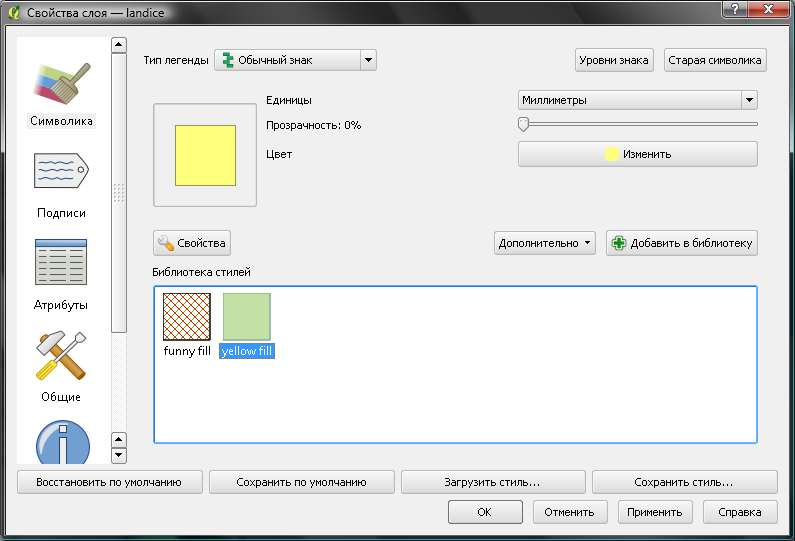
\includegraphics[clip=true, width=0.3\textwidth]{singlesymbol_ng_area}}
\caption{Опции отрисовки <<обычным знаком>> в новой символике \wincaption}
\end{figure}

\minisec{Отрисовка уникальными значениями}

Используется для отрисовки всех элементов слоя единым, определенным
пользователем, символом, цвет которого отражает значение выбранного
атрибута элемента. Вкладка символики позволяет вам выбрать:

\begin{itemize}[label=--]
\item Поле (в списке полей)
\item Знак (в диалоге <<Выбор условного знака>>)
\item Градиент (в списке цветовых шкал)
\end{itemize}

Для удобства список в нижней части вкладки показывает значения всех заданных
на данный момент атрибутов, включая символы, к которым в будущем
будет применена отрисовка.

Рисунок~\ref{fig:catsymNG} иллюстрирует диалог отрисовки уникальными значениями
на примере слоя рек из демонстрационного набора данных \qg.

\begin{figure}[ht]
   \centering
   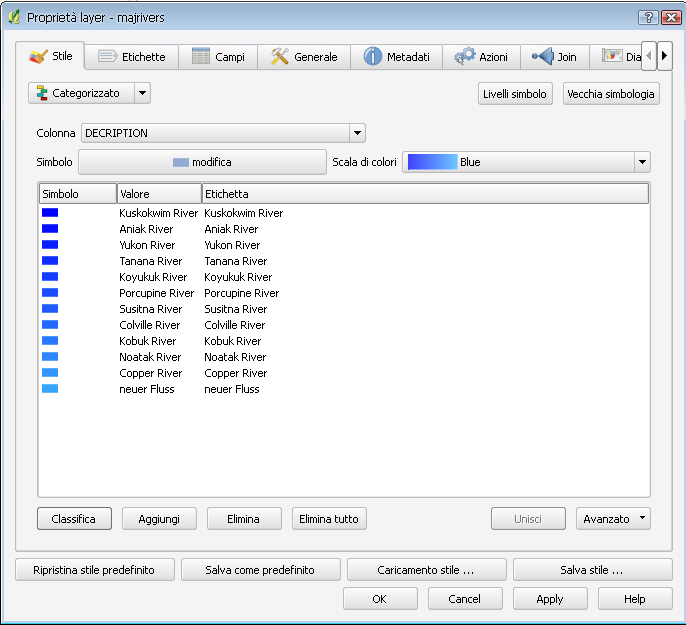
\includegraphics[clip=true, width=10cm]{categorysymbol_ng_line}
   \caption{Опции отрисовки <<уникальными значениями>> в новой символике \wincaption}\label{fig:catsymNG}
\end{figure}

\minisec{Отрисовка градуированным знаком}

Используется для рендеринга всех элементов слоя единым, определенным
пользователем, символом, цвет которого отражает соответствие
выбранного атрибута элемента некоторому классу.

Как и в случае отрисовки категориями, вкладка символики позволяет вам выбрать:

\begin{itemize}[label=--]
\item Поле (в списке полей)
\item Знак (в диалоге <<Выбор условного знака>>)
\item Градиент (в списке цветовых шкал)
\end{itemize}

Кроме этого, вы можете задать количество классов, а также режим классификации
элементов внутри класса (в списке режимов). Список в нижней части вкладки
символики содержит информацию о классах вместе с их диапазонами, подписями
и символами, которые будут использованы при отрисовке.

Рисунок \ref{fig:gradsymNG} иллюстрирует диалог отрисовки
<<градуированным знаком>> на примере слоя рек из демонстрационного набора данных \qg.

\begin{figure}[ht]
   \centering
   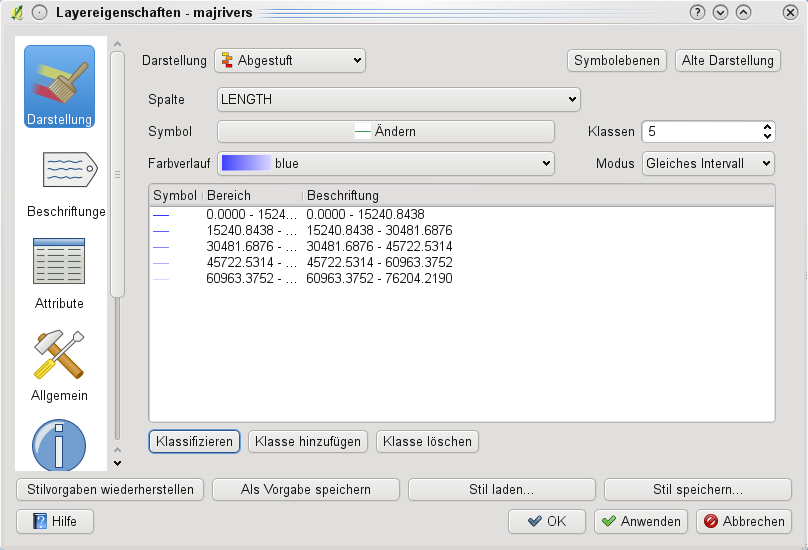
\includegraphics[clip=true, width=10cm]{graduatesymbol_ng_line}
   \caption{Опции  отрисовки <<градуированным знаком>> в новой символике \wincaption}\label{fig:gradsymNG}
\end{figure}

\minisec{Отрисовка на основе правил}

Используется для отрисовки всех элементов слоя с помощью символов,
базирующихся на определенных правилах. Цвет символов отражает
соответствие выбранного атрибута элемента некоторому классу.

%%FIXME Add more text here

Рисунок~\ref{fig:rulesymNG} иллюстрирует диалог отрисовки по заданным
<<правилам>> на примере слоя рек из демонстрационного набора данных \qg.

\begin{figure}[ht]
   \centering
   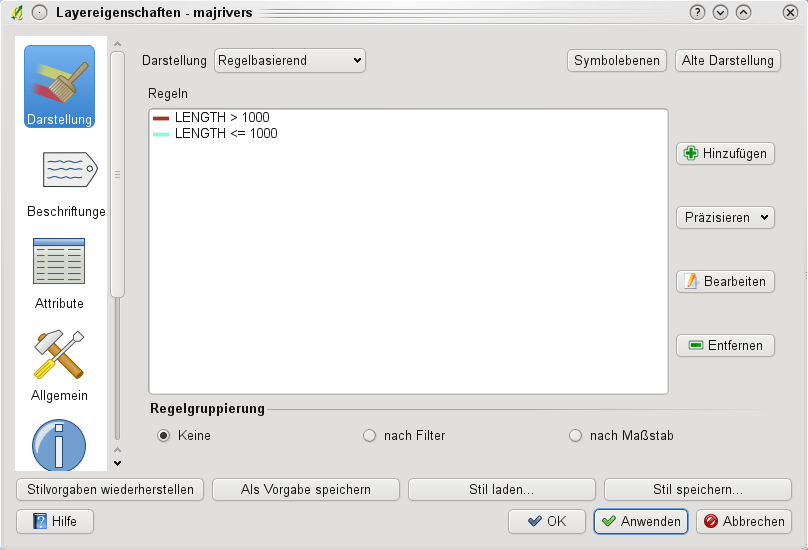
\includegraphics[clip=true, width=10cm]{rulesymbol_ng_line}
   \caption{Опции отрисовки <<по правилам>> в новой символике \wincaption}\label{fig:rulesymNG}
\end{figure}

\minisec{Свойства знака}

Диалог <<Свойства знака>> дает пользователю возможность задать различные
свойства для символа. В левой верхней части диалога (<<Предварительный
просмотр>>)  вы найдете уменьшенную копию текущего символа в том виде,
в котором он будет отображен на карте. Под уменьшенной копией расположен
список символьных слоёв (<<Слои условного знака>>) . Для открытия диалога
свойств символа нажмите кнопку \dropmenuopttwo{mActionOptions}{Свойства}
вкладки \tab{Символика} диалога \dialog{Свойства слоя}.

Панели инструментов дают возможность добавлять и удалять слои, изменять их
положение, а также, при необходимости, запретить их изменение
(<<Заблокировать цвет слоя>>). В правой части диалога показаны настройки,
применяемые к простому символьному слою из соответствующего списка. Наиболее
важной частью диалога является выпадающий список типов символьного слоя.
Список допустимых значений зависит от типа слоя (точечный, линейный,
полигональный).

\begin{description}
\item Опции типа условного знака для точечных слоёв
\begin{itemize}[label=--]
\item \textbf{Символьный маркер}: шрифт, цвет, размер, вращение
\item \textbf{Простой маркер}: цвет обводки, цвет заливки, размер, угол,
смещение по X,Y
\item \textbf{SVG-маркер}: размер, угол, смещение по X,Y; SVG-изображение
\end{itemize}
\item Опции типа условного знака для линейных слоёв
\begin{itemize}[label=--]
\item \textbf{Обрамление линии}: цвет
\item \textbf{Маркерная линия}: маркер, интервал маркеров, вращать
маркер, смещение линии
\item \textbf{Простая линия}: цвет, толщина линии, смещение, стиль
линии, пользовательский пунктир, соединение, концы
\end{itemize}
\item Опции типа условного знака для полигональных слоёв
\begin{itemize}[label=--]
\item \textbf{SVG-заливка}: ширина текстуры, обводка
\item \textbf{Простая заливка}: цвет, стиль заливки, цвет обводки,
стиль обводки, толщина обводки, смещение по X,Y
\end{itemize}
\end{description}


\begin{figure}[ht]
\centering
   \subfloat[Линия, образованная из трёх простых линий] {\label{subfig:symprops1}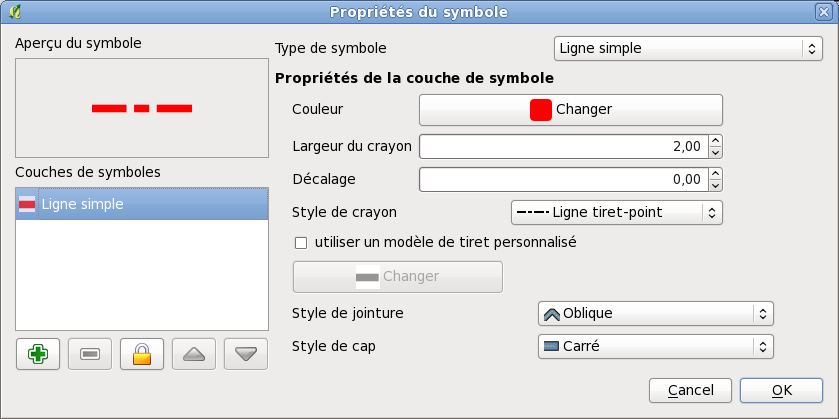
\includegraphics[clip=true, width=0.3\textwidth]{symbolproperties1}}
   \hspace{1cm}
   \subfloat[Свойства символа точечного слоя] {\label{subfig:symprops2}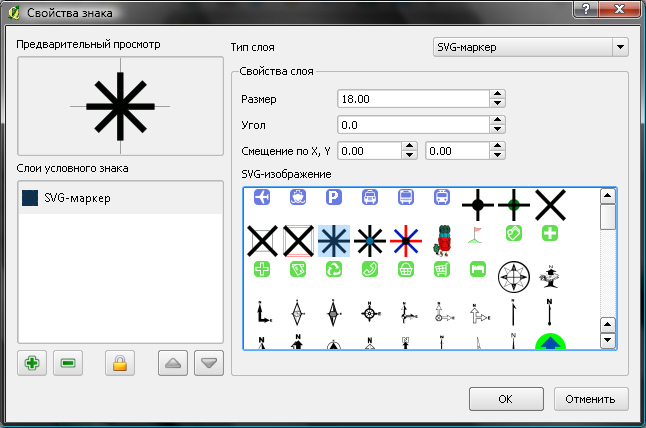
\includegraphics[clip=true, width=0.3\textwidth]{symbolproperties2}}
   \hspace{1cm}
   \subfloat[Шаблон заливки полигона] {\label{subfig:symprops3}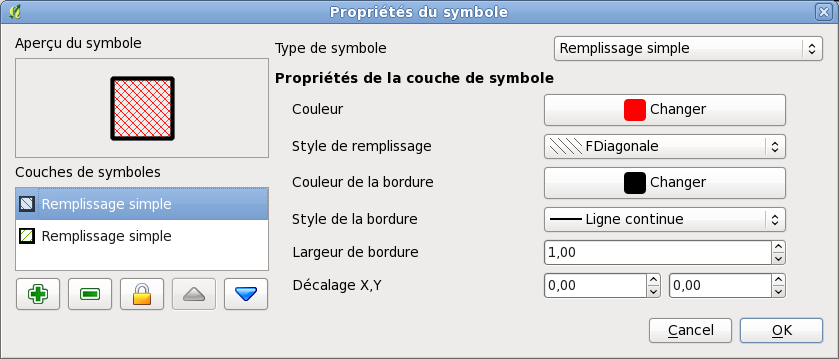
\includegraphics[clip=true, width=0.3\textwidth]{symbolproperties3}}
\caption{Задание свойств символа \wincaption}
\end{figure}

\subsection{Управление стилями}\label{subsec:stylemanager}

Менеджер стилей "--- это простое вспомогательное приложение, предоставляющее
пользователю доступные символы и цветовые шкалы для того или иного стиля.
Это приложение также позволяет добавлять и/или удалять элементы. Для его
запуска выберите пункт меню \mainmenuopt{Установки} \arrow
\dropmenuopt{Управление стилями}.

\begin{figure}[ht]
   \centering
   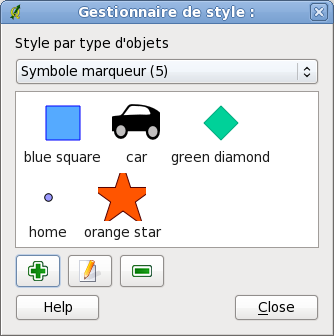
\includegraphics[clip=true, width=7cm]{stylemanager}
   \caption{Менеджер стилей для управления символами и цветовыми шкалами \wincaption}\label{fig:stylemanager}
\end{figure}

\subsection{Подписи}\label{labeltab}

Вкладка \tab{Подписи} позволяет подписывать объекты и контролировать
множество опций, касающихся шрифтов, расположения, стиля, выравнивания и
буферизации.

Чтобы продемонстрировать эти возможности, мы подпишем элементы слоя озер
из демонстрационного набора данных \qg:

\begin{enumerate}
\item Загрузите в \qg shape-файл \filename{alaska.shp} и GML-файл \filename{lakes.gml}.
\item Немного увеличьте интересующую вас область с каким-либо озером.
\item Сделайте слой \filename{lakes} активным.
\item Откройте диалог \dialog{Свойства слоя}.
\item Щёлкните на вкладке \tab{Подписи}.
\item Установите флажок \checkbox{Показывать подписи}.
\item Выберите поле, являющийся источником значений для подписей. В нашем
случае мы используем \selectstring{{}Поле, содержащее подпись}{NAMES}.
\item Введите значение по умолчанию, которое будет использоваться всякий
раз, когда \qg обнаружит озеро, у которого отсутствует значение в поле
\guilabel{NAMES}.
\item Если у вас имеются подписи, распространяющиеся на несколько линий,
установите флажок \\
\checkbox{Разбивать подписи на строки?} \qg проверит поле подписей на
наличие переходов на новую строку и вставит разрывы строк в нужных местах.
Переходом на новую строку считается \textbf{одиночный} символ <<\textbackslash n>>,
(а не два отдельных символа, такие, как символ обратного слеша <<\textbackslash >>
~за которым следует символ n).
\item Нажмите \button{Применить}.
\end{enumerate}

Теперь у нас есть подписи. Как они выглядят? Кажется, они слишком большие
и плохо размещены по отношению к маркерному символу озер.

Перейдите к области \tab{Шрифт} и установите шрифт и цвет с помощью кнопок
\button{Шрифт} и \button{Цвет}. Вы также можете изменить угол наклона и
расположение текста подписи.

Для смены позиции текста относительно элемента:

\begin{enumerate}
\item Измените расположение подписей, выбрав одну из кнопок группы \classname{Размещение}.
Для того, чтобы сделать подписи неподвижными, выберите кнопку \radiobuttonon{{}Справа}.
\item \classname{Единицы измерения размера шрифта} дают вам возможность
выбора между \radiobuttonon{{}Пунктами} и \radiobuttonon{{}Единицами карты}.
\item Нажмите кнопку \button{Применить}, чтобы увидеть результаты
изменений, не выходя из диалога.
\end{enumerate}

Смотрится лучше, но подписи все еще расположены слишком близко к маркеру.
Для того, чтобы исправить это, мы можем использовать опции области \tab{Смещение}.
Здесь мы можем добавить смещение по координатам X и Y. Смещение по координате
X на 5 единиц сдвинет подписи в сторону от маркеров и сделает их более
<<читаемыми>>. Естественно, если шрифт вашего маркерного символа больше,
то требуется и большее смещение.

Последняя настройка, которую мы сделаем, "--- добавим
\tab{Буферизовать подписи} к подписям. Под буферизацией подписей имеется
в виду всего лишь создание фона вокруг них для улучшения внешнего вида.
Чтобы буферизировать подписи, нужно:

\begin{enumerate}
\item Щёлкнуть на вкладке \tab{Параметры подписей}.
\item Установить флаг \checkbox{Буферизовать подписи}.
\item Выбрать размер буфера в счетчике.
\item Выбрать цвет, нажав на кнопку \button{Цвет} и выбрав желаемый в
окне выбора цвета. При желании можно установить нужное значение
прозрачности для буфера.
\item Нажать \button{Применить}, чтобы увидеть результат внесенных изменений.
\end{enumerate}

Если вы не удовлетворены результатами, измените настройки и протестируйте
снова, нажав кнопку \button{Применить}.

Буфер размером в 1~пункт обычно дает неплохой результат. Обратите внимание,
что вы можете также задать размер буфера в единицах измерения карты, если
вам кажется, что так будет лучше.

Оставшиеся области во вкладке \tab{Дополнительно} позволяют устанавливать
параметры подписей с использованием полей слоя.

Обратите внимание, что во вкладке \tab{Подписи} есть \classname{Предпросмотр:},
в котором показывается выбранная подпись.

\subsection{Новый стиль подписей}\index{новый стиль подписей}\label{newlabel}

Новое приложение ядра \qg \toolbtntwo{labeling}{Подписи} дает возможность
создать элегантные подписи для точечных, линейных и полигональных векторных
слоёв. Для его работы необходимо задание всего нескольких параметров.
Это новое приложение заменяет существующую функциональность подписей QGIS,
описанную в секции~\ref{labeltab}, а также поддерживает слои с преобразованием
<<на лету>>.

\minisec{Использование нового стиля подписей}

\begin{enumerate}
  \item Запустите QGIS и загрузите точечный, линейный или полигональный
  векторный слой.
  \item Сделайте слой активным в легенде и нажмите на иконку
  \toolbtntwo{labeling}{Подписи} в панели инструментов QGIS. Либо выберите
пункт меню \mainmenuopt{Слой} \arrow \dropmenuopt{Подписи}
\end{enumerate}

\minisec{Создание подписей для точечных слоёв}

Первым шагом является установка флага \checkbox{Подписывать объекты этого слоя}
и выбор атрибутивной колонки, используемой в качестве источника подписей.
После этого вы можете указать размещение подписи, её приоритет, стиль
текста, буферизацию текста, видимость подписи в пределах масштаба. Также
можно указать, необходимо ли подписывать части составных объектов и могут
ли подписи перекрывать объекты (см. Рисунок~\ref{fig:pointlabel}).

\begin{figure}[ht]
\centering
   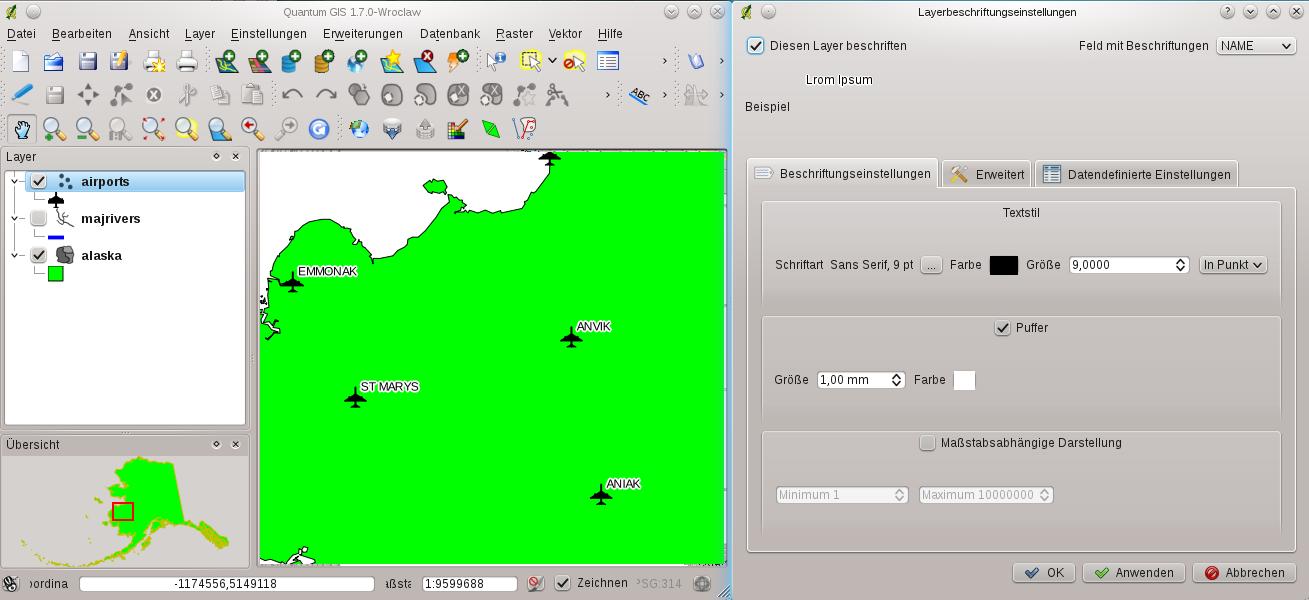
\includegraphics[clip=true, width=10cm]{label_points}
   \caption{Элегантные подписи для точечных векторных слоёв \wincaption}\label{fig:pointlabel}
\end{figure}

\minisec{Создание подписей для линейных слоёв}

Первым шагом является установка флага \checkbox{Подписывать объекты этого слоя}
и выбор атрибутивной колонки, используемой в качестве источника подписей.
После этого вы можете указать размещение подписи (в т.\,ч. её ориентацию),
её приоритет, стиль текста, буферизацию текста, видимость подписи в пределах
масштаба. Также можно указать, необходимо ли подписывать части составных
объектов, объединять ли связанные линии, и могут ли подписи перекрывать объекты
(см. Рисунок~\ref{fig:linelabel}).

\begin{figure}[ht]
\centering
   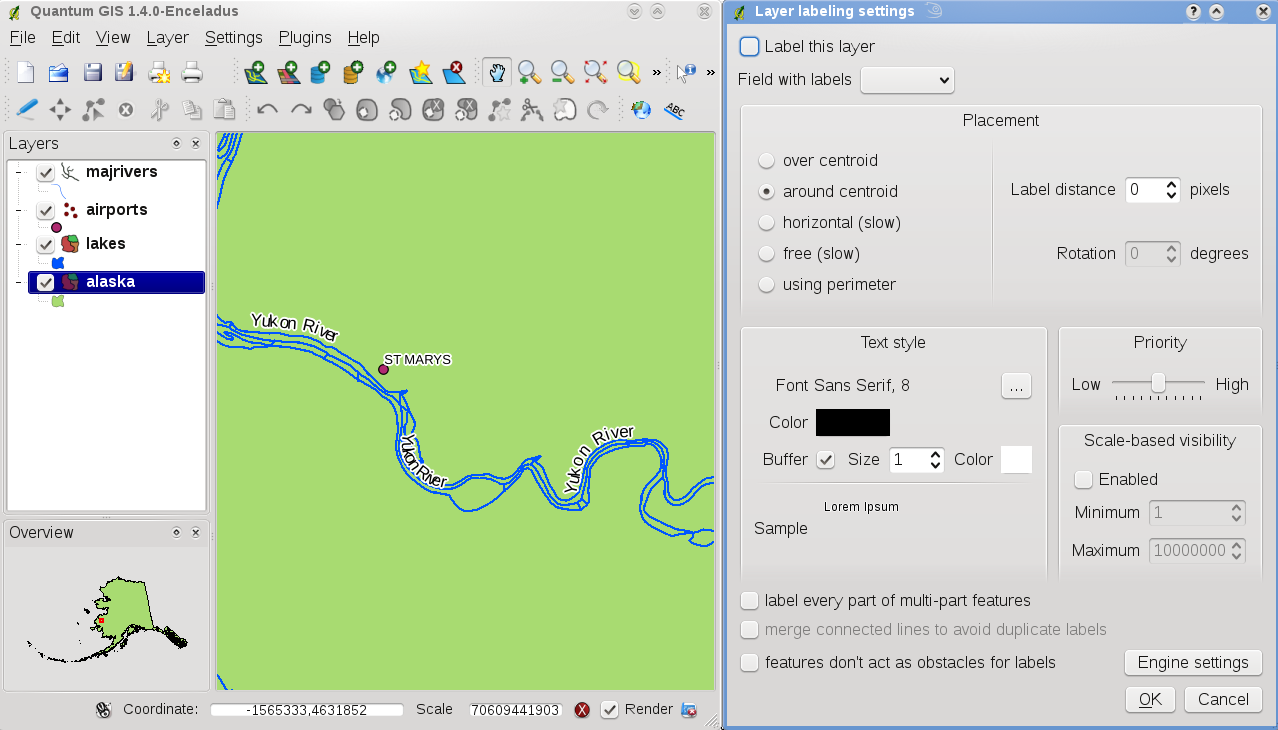
\includegraphics[clip=true, width=10cm]{label_line}
   \caption{Элегантные подписи для линейных векторных слоёв \wincaption}\label{fig:linelabel}
\end{figure}

\minisec{Создание подписей для полигональных слоёв}

Первым шагом является установка флага \checkbox{Подписывать объекты этого слоя}
и выбор атрибутивной колонки, используемой в качестве источника подписей.
После этого вы можете указать размещение подписи, её приоритет, стиль
текста, буферизацию текста, видимость подписи в пределах масштаба. Также
можно указать, необходимо ли подписывать части составных объектов и могут
ли подписи перекрывать объекты (см. Рисунок~\ref{fig:arealabel}).

\begin{figure}[ht]
\centering
   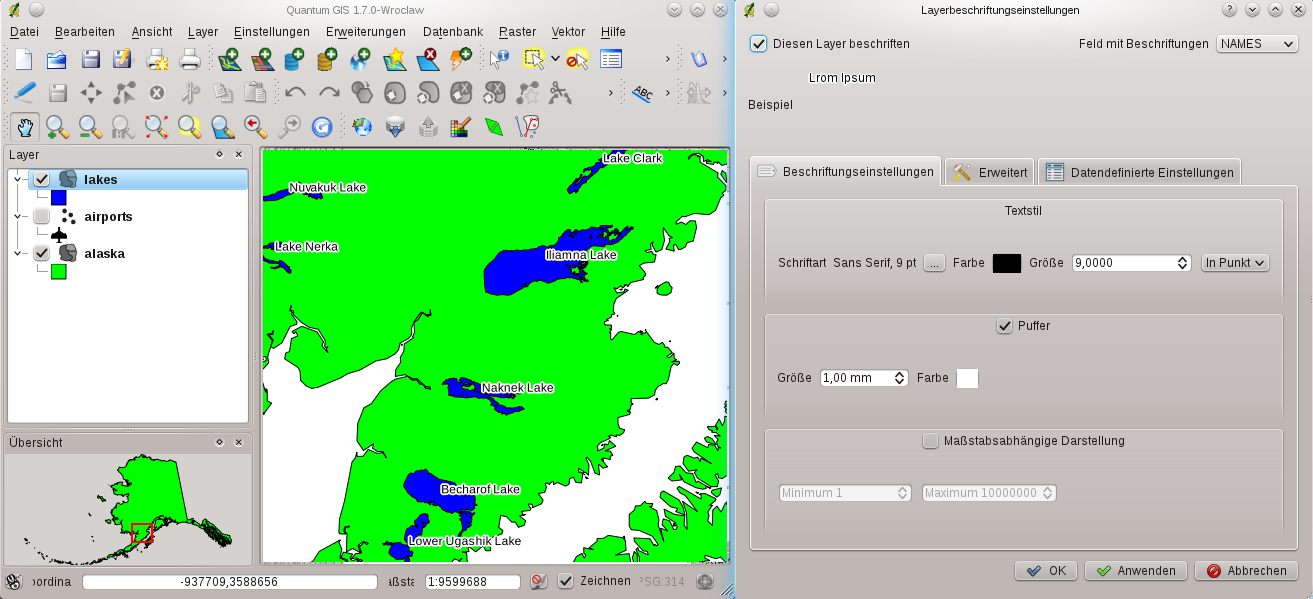
\includegraphics[clip=true, width=10cm]{label_area}
   \caption{Элегантные подписи для площадных векторных слоёв \wincaption}\label{fig:arealabel}
\end{figure}

\minisec{Изменение параметров алгоритма размещения подписей}

Вы также можете нажать кнопку \button{Параметры алгоритма} и выбрать метод,
используемый для поиска наилучшего места для подписи. Доступные методы:
Chain, Popmusic Tabu, Popmusic Chain, Popmusic Tabu Chain и FALP.

\begin{figure}[ht]
\centering
   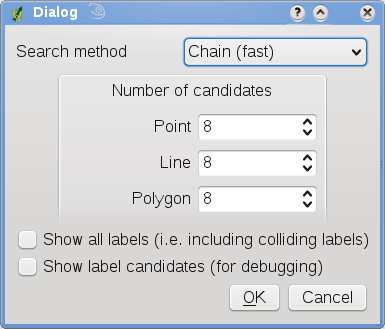
\includegraphics[clip=true, width=5cm]{label_engine}
   \caption{Диалог изменения параметров алгоритма размещения подписей \wincaption}\label{fig:labelengine}
\end{figure}

Более того, можно задать количество возможных подписей при данном методе
поиска отдельно для точечных, линейных и полигональных элементов, а также
необходимо ли показывать все подписи (включая перекрывающиеся подписи) и
необходимо ли показывать возможные подписи (для отладки).

\subsection{Атрибуты}\index{атрибуты}\label{label_attributes}

Во вкладке \tab{Атрибуты} можно изменять атрибуты выбранного набора данных.
Кнопки \toolbtntwo{mActionNewAttribute}{Добавить поле} и
\toolbtntwo{mActionDeleteAttribute}{Удалить поле} можно использовать, если
данные находятся в \toolbtntwo{mActionToggleEditing}{Режиме редактирования}.
В данный момент можно удалять и добавлять только поля слоёв PostGIS.
Библиотека OGR позволяет добавлять новые поля, но не удалять их, если
у вас установлена версия GDAL >= 1.6.

\minisec{Элемент редактирования}

\begin{figure}[ht]
   \centering
   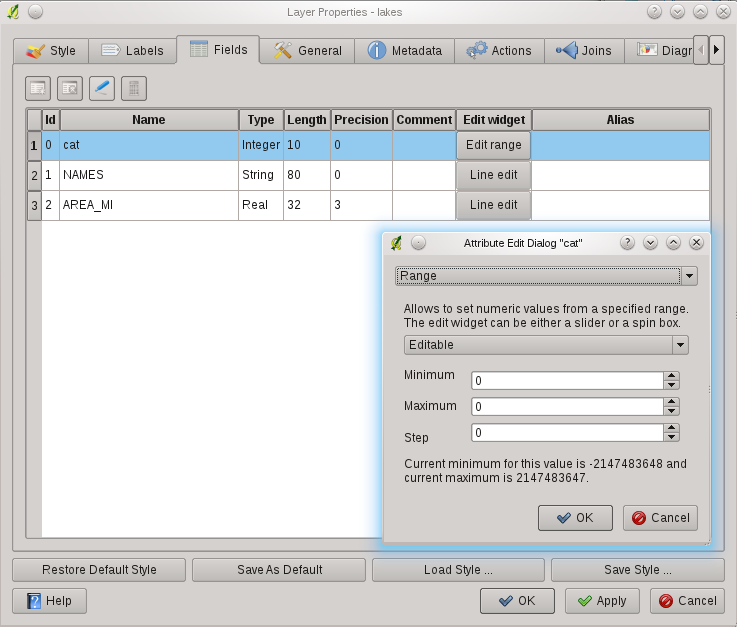
\includegraphics[clip=true, width=12cm]{editwidgetsdialog}
   \caption{Диалог выбора элемента редактирования поля
\wincaption}\label{fig:editwidget}
\end{figure}

Во вкладке \tab{Атрибуты} вы также можете найти колонку
\texttt{Элемент редактирования}. Эта колонка может использоваться для
задания значений или диапазона значений, которые можно присваивать
конкретному полю таблицы. При нажатии кнопки \button{Элемент редактирования}
открывается диалог, в котором можно задать различные элементы. Среди них:

\begin{itemize}[label=--]
\item Строчное редактирование: Поле, позволяющее вводить простой текст
(или числа для числовых атрибутов).
\item Классификация: Отображает выпадающий список значений, используемых для
классификации, если вы выбрали <<Уникальные значения>> в качестве типа легенды
во вкладке символики.
\item Диапазон: Позволяет вводить числовые значения из указанного
диапазона. Элемент редактирования может быть либо <<ползунком>>, либо
полем ввода.
\item Уникальные значения: Пользователь может выбрать одно из значений, уже
используемых для атрибута. Если активирован параметр <<Поле ввода>>, то
будет использоваться поле ввода с автодополнением, иначе будет использоваться
выпадающий список.
\item Имя файла: Упрощает процесс выбор файлов за счёт добавления
соответствующего диалога.
\item Карта значений: Выпадающий список с предопределенными значениями.
Значение сохраняется в атрибуте, описание выводится в списке.
\item Перечень: Выпадающий список значений, допустимых для данного типа
поля. На данный момент эта функциональность доступна только для слоёв PostGIS.
\item Неизменяемый: Неизменяемый атрибут нельзя редактировать (он
доступен только для чтения).
\item Скрытый: Скрытый атрибут не будет виден пользователю.
\item Флажок: Значение для активированного состояния, значение для
неактивированного состояния.
\item Текстовое поле: Текстовое поле, позволяющее ввод многострочного текста.
\item Календарь: Календарь для ввода даты.

\end{itemize}

\subsection{Общие}\label{vectorgeneraltab}

Вкладка \tab{Общие} очень схожа с аналогичной вкладкой диалога свойств
растрового слоя. Она позволяет изменять отображаемое в легенде имя слоя,
устанавливать диапазон масштабов, при которых производится отрисовка,
создавать пространственный индекс для векторного файла (только для форматов,
поддерживаемых OGR, и PostGIS), просматривать или изменять проекцию
определенного векторного слоя.

Кнопка \button{Конструктор запросов} позволяет создать подмножество
элементов слоя. конструктор запросов доступен также, когда вы
открываете таблицу атрибутов и нажимаете кнопку \button{Расширенный поиск}.

\subsection{Метаданные}\index{метаданные}

Вкладка \tab{Метаданные} содержит общую информацию о слое, включая
специфическую информацию о типе хранилища и источнике слоя, типе
геометрии и количестве объектов слоя,  возможностях редактирования
слоя. Раздел \guiheading{Границы} предоставляет
информацию о границах содержимого слоя, а раздел
\guiheading{Система координат слоя} предоставляет информацию о его
системе координат. Это быстрый способ получить информацию о слое, но
редактирование метаданных пока еще невозможно .

\subsection{Действия}\index{действия}\label{label_actions}

\qg позволяет выполнять действия с использованием атрибутов элемента. Эту
вкладку можно использовать для выполнения любого количества действий, например,
запуск программы с параметрами, взятыми из атрибутов элемента, или передача
параметров в веб-утилиту генерации отчётов.

Действия могут быть полезными при частом запуске внешнего приложения или
просмотра веб-страницы, которая зависит от одного или нескольких значений
вашего векторного слоя. Примером может служить выполнение поиска по
значению атрибута. Эта концепция обсуждается ниже.

\minisec{Задание действий}\index{действия!задание}

Действия с использованием атрибутов задаются в диалоге \dialog{Свойства слоя}.
Чтобы задать действие, откройте диалог \dialog{Свойства слоя} векторного
слоя и перейдите во вкладку \tab{Действия}. Укажите наглядное имя для
действия. Действие само по себе должно содержать имя приложения, которое
запустится при вызове действия. Вы можете добавить одно или
несколько атрибутивных полей в качестве аргументов запускаемого приложения.
Когда действие вызовется, любое множество символов, начинающихся с \%, за
которым следует имя поля, будет заменено на соответствующее значение
этого поля. Специфические символы \%\% \index{\%\%} заменяются значением поля,
которое выбирается из результатов идентификации или атрибутивной таблицы
(см. Раздел <<Использование действий>>). Для группировки текста в
единый аргумент программы, скрипта или команды можно использовать двойные кавычки.
Двойные кавычки игнорируются в случае, если им предшествует символ обратного
слеша.

Если какие-то из имен полей являются подстроками других имен полей (например,
\usertext{col1} и \usertext{col10}), вам следует указать это, заключив имя
поля (и символ \%) в квадратные скобки (например, \usertext{[\%col10]}).
Это позволит не путать поле \usertext{\%col10} с полем \usertext{\%col1} и
\usertext{0} на конце. \qg удаляет скобки во время замены названия поля
на его значение. Если вы хотите, чтобы замещенное поле было заключено
в квадратные скобки, используйте сигнатуру наподобие этой: \usertext{[[\%col10]]}.

Диалог \dialog{Результаты идентификации} включает в себя элемент {\em (Выведенные)},
содержащий соответствующую типу слоя информацию. Значения этого элемента
можно получить схожим с другими полями образом "--- поставив перед именем
наследуемого поля \usertext{(Выведенные).}. Например, точечный слой имеет поля
\usertext{X} и \usertext{Y}, значения этих полей можно использовать в действии
в качестве параметров \usertext{\%(Выведенные).X} и \usertext{\%(Выведенные).Y}.
Наследуемые атрибуты доступны только из диалога \dialog{Результаты идентификации},
и, соответственно, недоступны из диалога \dialog{Таблица атрибутов}.

Покажем два тестовых действия:\index{действия!примеры} (\nix, KDE )

\begin{itemize}[label=--]
  \item \usertext{konqueror http://www.google.com/search?q=\%nam}
  \item \usertext{konqueror http://www.google.com/search?q=\%\%}
\end{itemize}

В первом примере вызывается веб-браузер konqueror и передается URL, который
необходимо в нем открыть. URL выполняет поиск в Google по значению поля
\usertext{nam} нашего векторного слоя. Обратите внимание, что запускаемое
приложение или вызываемый скрип должны находиться в текущей директории,
иначе вы должны указывать полный путь. Чтобы убедиться, что действие
выполнится правильно, мы можем переписать первый пример как:
\usertext{/usr/bin/konqueror http://www.google.com/search?q=\%nam}. Это
обеспечит запуск приложения konqueror при вызове действия.

Второй пример использует нотацию \%\%, которая не замещает ни одно поле
его значением. Когда действие вызывается, \%\% замещается значением выбранного
поля результатов идентификации или таблицы атрибутов.

\minisec{Использование действий}\index{действия!использование}\label{label_usingactions}

Действия вызываются либо из диалогов \dialog{Результаты идентификации} или
\dialog{Таблица атрибутов} (вызвать эти диалоги можно, нажав на
\toolbtntwo{mActionIdentify}{Определить объекты} или
\toolbtntwo{mActionOpenTable}{Открыть таблицу атрибутов}). Чтобы вызвать
действие, щёлкните правой кнопкой мыши на записи и выберите действие из
контекстного меню. Действия указаны в контекстном меню с именами, которые
вы им назначили во время задания действий. Щёлкните на действии, которое
вы хотите вызвать.

Если вы вызываете действие, использующее нотацию \%\%, выполните правый
щелчок на значении поля, которое вы хотите передать приложению или скрипту,
в диалоге \dialog{Результаты идентификации} или в диалоге \dialog{Таблица
атрибутов}.

Здесь приведен другой пример, иллюстрирующий процесс записи данных векторного
слоя в файл с использованием bash и комманды \usertext{echo} (так что он
будет работать только в \nix или (возможно) \osx). Используемый в примере
слой имеет поля имени \usertext{taxon\_name}, широты \usertext{lat} и долготы
\usertext{long}. Для того чтобы записать значения этих полей в текстовый файл,
необходимо вызвать следующее действие:

\begin{verbatim}
  bash -c "echo \"%taxon_name %lat %long\" >> /tmp/species_localities.txt"
\end{verbatim}

После вызова этого действия для нескольких записей таблицы, результирующий
файл будет выглядеть примерно так:

\begin{verbatim}
  Acacia mearnsii -34.0800000000 150.0800000000
  Acacia mearnsii -34.9000000000 150.1200000000
  Acacia mearnsii -35.2200000000 149.9300000000
  Acacia mearnsii -32.2700000000 150.4100000000
\end{verbatim}

В качестве упражнения мы создадим действие, выполняющее поиск в Google по
слою \filename{lakes}. Для начала, нам необходимо указать URL, необходимый
для выполнения поиска по ключевому слову. Это легко сделать, просто перейдя
на сайт Google и выполнив простой поиск, затем необходимо скопировать URL
из адресной строки вашего браузера. Итак, мы видим, что формат имеет вид:
\url{http://google.com/search?q=qgis}, где \usertext{\qg} "--- это ключевое
слово поиска. Имея в виду эту информацию, мы можем продолжать:

\begin{enumerate}
\item Убедитесь, что слой \filename{lakes} загружен.
\item Откройте диалог \dialog{Свойства слоя}, сделав двойной щелчок на слое в
легенде или щёлкнув правой кнопкой мыши и выбрав \dropmenuopt{Свойства} в
контекстном меню.
\item Перейдите на вкладку \tab{Действия}.
\item Введите имя действия, например, \usertext{Google Search}.
\item Для действия нам нужно задать имя внешней запускаемой программы.
В этот раз мы будем использовать веб-браузер Firefox. Если программы нет в текущей
директории, необходимо задать полный путь к ней.
\item Следом за именем внешнего приложения добавьте URL, используемый для
выполнения поиска в Google (но не указывайте параметр поиска):
\url{http://google.com/search?q=}
\item Теперь текст в поле \guilabel{Действие} должен выглядеть так:\\
\usertext{firefox \url{http://google.com/search?q=}}
\item Щёлкните на выпадающем списке, содержащем имена полей
слоя \usertext{lakes}. Он расположен непосредственно слева от кнопки
\button{Вставить поле}.
\item Выберите в списке \selectstring{{}Поле, содержащее подписи}{NAMES} и
нажмите \button{Вставить поле}.
\item Теперь текст вашего действия выглядит так:\\
\usertext{firefox \url{http://google.com/search?q=\%NAMES}}
\item И, наконец, нажмите кнопку \button{Вставить действие}.
\end{enumerate}

Теперь действие создано и готово к использованию. Окончательный текст
действия должен выглядеть так:

\usertext{firefox \url{http://google.com/search?q=\%NAMES}}

Теперь мы можем использовать это действие. Закройте диалог \dialog{Свойства слоя}
и приблизьтесь к области интереса. Убедитесь, что слой \filename{lakes}
активный и выберите озеро. В окне результатов вы теперь видите, что ваше
действие показывается:

\begin{figure}[ht]
   \centering
   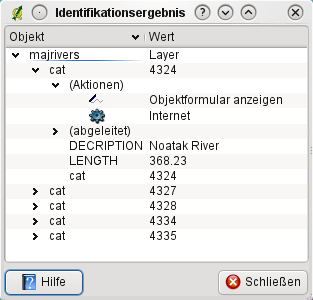
\includegraphics[clip=true, width=7cm]{action_identifyaction}
   \caption{Выделите элемент и выберите действие \wincaption}\label{fig:identify_action}
\end{figure}

Во время вызова действия запустится Firefox и откроется URL
\url{http://www.google.com/search?q=Tustumena}. Также возможно добавить
дополнительные поля к действию. Следовательно, вы можете добавить <<+>>
в конец текста действия, выбрать другое поле и нажать кнопку
\button{Вставить поле}. В нашем примере более нет доступных полей, по которым
был бы смысл проводить поиск.

Вы можете задать несколько действий для слоя и каждое из них будет показано в
диалоге \\
\dialog{Результаты идентификации}.
%% FIXME No longer valid??
%%You can also invoke actions from the attribute table
%%by selecting a row and right-clicking, then choosing the action from the popup
%%menu.

Существует множество применений действий. Например, если у вас есть точечный
слой, который содержит информацию о пути к изображениям или фото, вы можете
создать действие запуска приложения, с помощью которого можно просматривать
изображения. Вы также можете использовать действия для генерации веб-отчётов
об атрибутивном поле или комбинации полей, задавая их в схожей манере, как
мы это делали в примере поиска в Google.

\subsection{Наложение диаграмм}\label{sec:diagram}
\index{векторные слои!диаграммы}

Вкладка \tab{Наложение диаграмм} позволяет вам осуществлять наложение графики на
векторный слой. Чтобы сделать эту функцию доступной, откройте <<Менеджер модулей>>
и выберите модуль <<Наложение диаграмм>>. После этого в диалоге \dialog{Свойства слоя}
векторного слоя появится новая вкладка, в которой можно задать настройки диаграмм
(см. Рисунок~\ref{fig:diagramtab}).

\begin{figure}[ht]
   \centering
   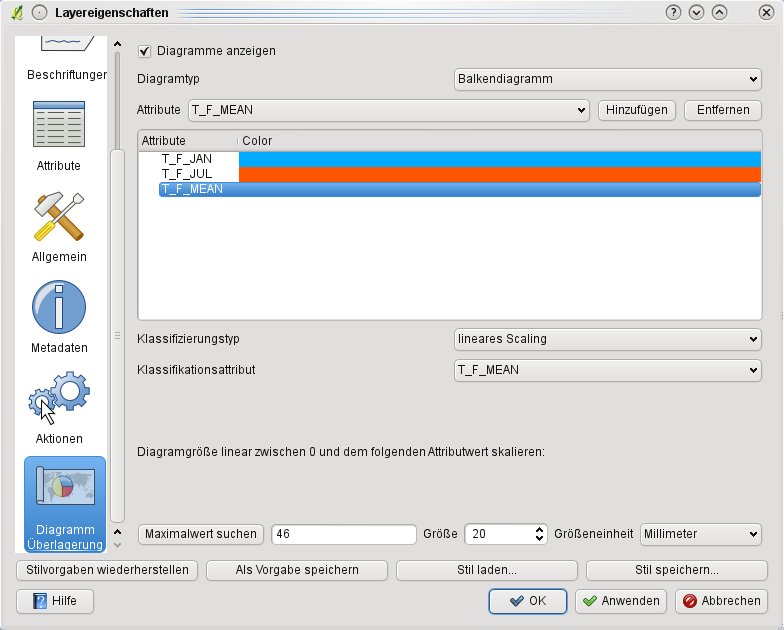
\includegraphics[clip=true, width=13cm]{diagram_tab}
   \caption{Диалог свойств векторного слоя с вкладкой <<Наложение диаграмм>> \wincaption}\label{fig:diagramtab}
\end{figure}

Текущая реализация предоставляет поддержку круговых диаграмм,
столбчатых диаграмм, пропорциональных SVG-символов, а также линейного масштабирования в зависимости
от атрибута классификации. Мы продемонстрируем пример наложения
столбчатой диаграммы некоторых климатических температурных данных
векторного слоя <<climate>> на cлой <<alaska>>.
Оба векторных слоя являются частью демонстрационного набора данных \qg
(см. Раздел~\ref{label_sampledata}).

\begin{enumerate}
\item Для начала нажмите на иконку \toolbtntwo{mActionAddOgrLayer}{Загрузить векторный слой},
просмотрите директорию демонстрационного набора данных \qg и загрузите два слоя
\filename{alaska.shp} и \filename{climate.shp}.
\item Сделайте двойной щелчок на слое \filename{climate} в легенде карты
и откройте диалог \dialog{Свойства слоя}.
\item Перейдите во вкладку \tab{Наложение диаграмм}, нажмите флажок
  <<Включить диаграммы>>, затем выберите
\button{Столбчатая} в качестве типа диаграммы.
\item Мы хотим отображать значения трёх колонок в диаграмме
\filename{T\_F\_JAN, T\_F\_JUL} и \filename{T\_F\_MEAN}. Для начала выберите
\filename{T\_F\_JAN} в качестве атрибута и нажмите кнопку \button{Добавить атрибут},
затем \filename{T\_F\_JUL} и, наконец, \filename{T\_F\_MEAN}.
\item Для линейного масштабирования размера диаграммы мы зададим \filename{T\_F\_JUL}
в качестве атрибута классификации.
\item Теперь нажмите на кнопку \button{Найти максимальное значение}, выберите
значение размера и единицы измерения, и нажмите кнопку \button{Применить} для
отображения диаграммы в главном окне \qg.
\item Теперь можно настроить размер диаграммы или изменить цвет атрибутов,
сделав двойной щелчок на значениях цветов в поле атрибутов. Смотрите
Рисунок~\ref{fig:climatediagram} в качестве иллюстрации.
\item Наконец, нажмите кнопку \button{Ok}.
\end{enumerate}

\begin{figure}[ht]
   \centering
   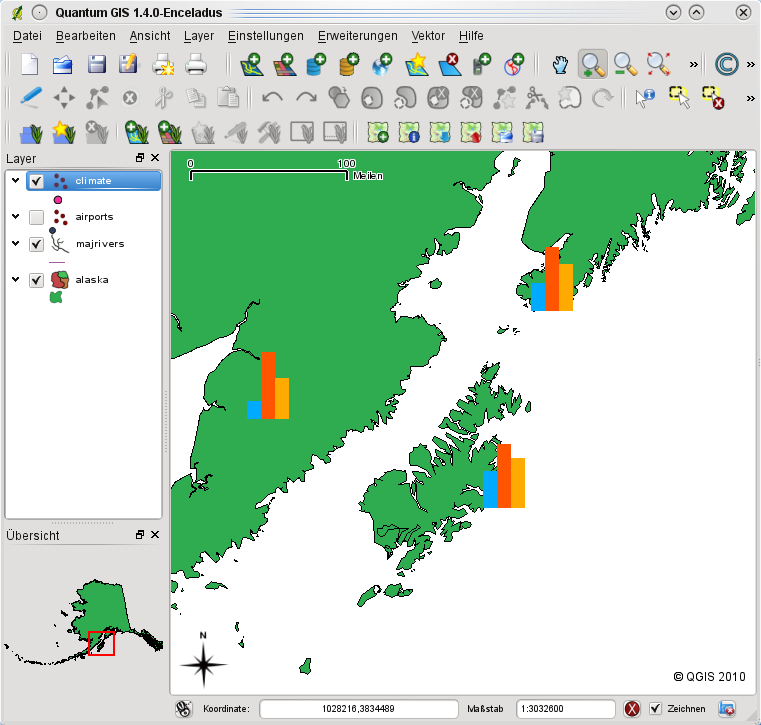
\includegraphics[clip=true, width=13cm]{climate_diagram}
   \caption{Диаграмма температурных данных, наложенная на карту \wincaption}\label{fig:climatediagram}
\end{figure}

\section{Редактирование}\index{редактирование}

\qg предоставляет разнообразные возможности для редактирования векторных
данных OGR, PostGIS и Spatialite. \textbf{Примечание} "--- процедура
редактирования данных GRASS имеет свои отличия "--- подробнее см.
Раздел~\ref{grass_digitising}.

\begin{Tip}\caption{\textsc{Параллельное редактирование}}
Данная версия \qg не различает между собой нескольких пользователей,
одновременно редактирующих одни и те же данные. Сохраняются изменения
того пользователя, который сохранил их последним.
\end{Tip}

\subsection{Настройка порога прилипания и радиуса поиска}\label{snapping_tolerance}

Перед началом редактирования узлов необходимо установить величину порога
прилипания и радиуса поиска, что позволит оптимизировать редактирование
геометрии векторных слоёв.

\minisec{Порог прилипания}

Порог прилипания "--- это расстояние, используемое \qg для \usertext{поиска}
ближайшего узла и/или сегмента, к которому надо присоединиться при создании
нового узла или передвижении уже существующего. Если превысить порог
прилипания, то при нажатии кнопки мыши узел будет создан <<в стороне>>,
вместо того, чтобы быть привязанным к уже существующему узлу и/или сегменту.
Величина порога прилипания оказывает влияние на функционирование всех
инструментов программы, связанных с величинами допуска.

\begin{enumerate}
\item Общая для всего проекта величина порога прилипания устанавливается в
\mainmenuopt{Установки} \arrow \dropmenuopttwo{mActionOptions}{Параметры}
(Для Mac: \mainmenuopt{\qg} \arrow Настройки, для Linux: \mainmenuopt{Редактирование}
\arrow \\ \dropmenuopttwo{mActionOptions}{Параметры}).
На вкладке \tab{Оцифровка} можно установить режим прилипания по
умолчанию: к вершинам, к сегментам, или к вершинам и сегментам. Также можно определить
значения по умолчанию для единиц измерения порога прилипания и радиуса поиска.
Эти величины  могут быть установлены как в единицах карты, так и в пикселах.
Преимущество использования пикселов в качестве единиц заключается в том, что
при зуммировании порог прилипания не будет изменяться.
В нашем небольшом проекте оцифровки (по рабочему набору данных Alaska) мы
установили в качестве единицы порога прилипания фут. Ваши результаты могут
отличаться, но величины, близкие к 300~футов, дают приемлемые
результаты при работе в масштабе 1:10~000.
\item Величина порога прилипания для отдельного слоя устанавливается в
\mainmenuopt{Установки} (или \mainmenuopt{Файл}) \arrow
\dropmenuopttwo{mActionOptions}{Свойства проекта\dots}. На вкладке \tab{Общие},
в секции \classname{Оцифровка} нажмите на \\
\button{Параметры прилипания\dots} для
включения и настройки режима и порога прилипания для каждого слоя (см.
Рисунок~\ref{fig:snappingoptions}).
\end{enumerate}
Обратите внимание, что величина порога прилипания для отдельного слоя
доминирует над общим порогом прилипания, установленным на вкладке \tab{Оцифровка}.
Таким образом, если надо отредактировать один слой и прилепить его вершины
к другому слою, необходимо активировать прилипание \usertext{прилипание к}
для слоя, затем снизить общий порог прилипания для проекта до меньшего
значения. Кроме того, прилипание невозможно для слоя, не активизированного
в диалоговом окне параметров прилипания, независимо от параметров
общего прилипания. Поэтому необходимо убедиться, что у слоя, к которому
необходимо применить прилипание, стоит флажок.

\begin{figure}[ht]
   \centering
   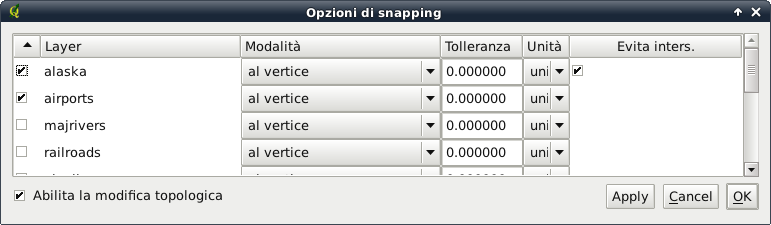
\includegraphics[clip=true, width=12cm]{editProjectSnapping}
   \caption{Установка параметров прилипания для отдельного слоя \wincaption}\label{fig:snappingoptions}
\end{figure}

\minisec{Радиус поиска}

Радиус поиска "--- это расстояние, используемое \qg для \usertext{поиска}
ближайшей вершины, которую вы пытаетесь переместить, щелкая кнопкой мыши
по карте. За пределом радиуса поиска \qg не сможет найти и выделить
какую-либо вершину для последующего редактирования, о чем сообщит
всплывающее окно предупреждения. Порог прилипания и радиус поиска
устанавливаются в единицах карты или пикселях, для того, чтобы установить
приемлемые значения, лучше всего с ними поэкспериментировать. Если установлен
слишком большой порог, \qg может прилепиться к неверной вершине, особенно,
если работа идет с большим количеством близко расположенных вершин. Однако
слишком маленький порог не позволит обнаружить какой-либо объект.

Радиус поиска для редактирования вершин в единицах слоя устанавливается
на вкладке \tab{Оцифровка}, расположенной в меню \mainmenuopt{Установки}
\arrow \dropmenuopttwo{mActionOptions}{Параметры}. Там же устанавливается
общий для всего проекта порог прилипания.

\subsection{Масштабирование и прокрутка карты}

Перед редактированием слоя следует увеличить район исследований на карте.
Это спасёт от ожидания прорисовки всех вершин слоя.

Помимо использования кнопок \toolbtntwo{mActionPan}{Прокрутка карты} и
\toolbtntwo{mActionZoomIn}{Увеличить}/\toolbtntwo{mActionZoomOut}{Уменьшить}
на панели инструментов, навигация также может осуществляться с
помощью <<колеса>> мыши, клавиши <<Пробел>> и стрелок.

\minisec{Зуммирование и прокрутка карты с помощью <<колеса>> мыши}

Нажатие и удержание <<колеса>> мыши во время редактирования позволяет перемещать
карту в пределах основного окна, а его прокручивание приводит к
масштабированию карты. Для увеличения необходимо расположить курсор мыши внутри
площади карты и крутить <<колесо>> вперед (от себя), для уменьшения "--- назад
(к себе). Положение курсора мыши является центром области зуммирования. Можно
настроить режим зуммирования <<колесом>> мыши, используя вкладку
\tab{Инструменты} в меню \mainmenuopt{Установки} \arrow \dropmenuopt{Параметры}.

\minisec{Прокрутка карты с помощью стрелок}

Прокрутка карты во время редактирования возможна с помощью стрелок. Расположите
курсор мыши внутри площади карты и нажмите на правую стрелку для перемещения на
восток, на левую стрелку для перемещения на запад, стрелку вверх для перемещения на
север и стрелку вниз для перемещения на юг.

Также возможно использовать клавишу «Пробел» для временного замещения мыши при
прокрутке карты. Нажатие стрелок клавиатуры «Вверх» и «Вниз» приведет к
увеличению и уменьшению карты, не прерывая процесса оцифровки.

\subsubsection{Топологическое редактирование}

Кроме установки параметров прилипания для отдельного слоя, на вкладке \tab{Общее}
из меню
\mainmenuopt{Установки} \arrow \dropmenuopttwo{mActionOptions}{Свойства проекта\dots}
можно установить топологическое редактирование. В группе опций по Оцифровке
можно активировать \checkbox{Включить топологическое редактирование} и/или
также активировать \\
\checkbox{Предотвращать пересечение новых полигонов}.

\minisec{Включение топологического редактирования}

Опция \checkbox{Включить топологическое редактирование} предназначена для
редактирования и управления общими границами в мозаике полигонов. \qg
«определяет» общие границы в мозаике полигонов. При изменении положения
вершины одного полигона \qg позаботится о том, чтобы положение вершины
соседнего полигона изменилось соответственно.

\minisec{Предотвращение пересечения новых полигонов}

Следующая топологическая опция называется \checkbox{Предотвращение пересечения
новых полигонов} и позволяет избежать пересечений в мозаике полигонов, что
ускоряет редактирование смежных полигонов. Если один полигон уже существует,
с помощью этой функции можно оцифровать новый с пересечением первого, и
\qg обрежет второй полигон по общей границе. Основное преимущество заключается
в том, что пользователи не должны цифровать все вершины по границе смежных
полигонов.

\subsection{Редактирование существующего слоя}
\index{векторные слои!оцифровка}
\index{оцифровка!существующего слоя}
\label{sec:edit_existing_layer}

По умолчанию, \qg подгружает слои, делая их доступными только для чтения:
это защита от непреднамеренного редактирования слоя, что случается, например,
при неловком движении <<мышкой>>. Однако, можно установить редактирование любого слоя
при условии, если на это имеется соответствующее разрешение, и основной
источник данных имеет возможность записи (т.\,е. эти файлы доступны не только
для чтения). Редактирование слоев наиболее универсально, если используются
источники данных, основанных на PostgreSQL/PostGIS.

Все возможности редактирования векторных слоев разделены между панелями
инструментов оцифровки и дополнительным функциям оцифровки, описанных в
Разделе~\ref{sec:advanced_edit}. Их можно активировать и деактивировать
в меню \mainmenuopt{Вид} \arrow \dropmenuopt{Панели инструментов}.
Используя основные инструменты для оцифровки, можно выполнять следующие
функции:

\begin{table}[ht]\index{векторные слои!основные инструменты редактирования}
\centering
\begin{tabular}{|l|p{5.5cm}|l|p{5.5cm}|}
\hline \textbf{Иконка} & \textbf{Назначение} & \textbf{Иконка} & \textbf{Назначение} \\
\hline 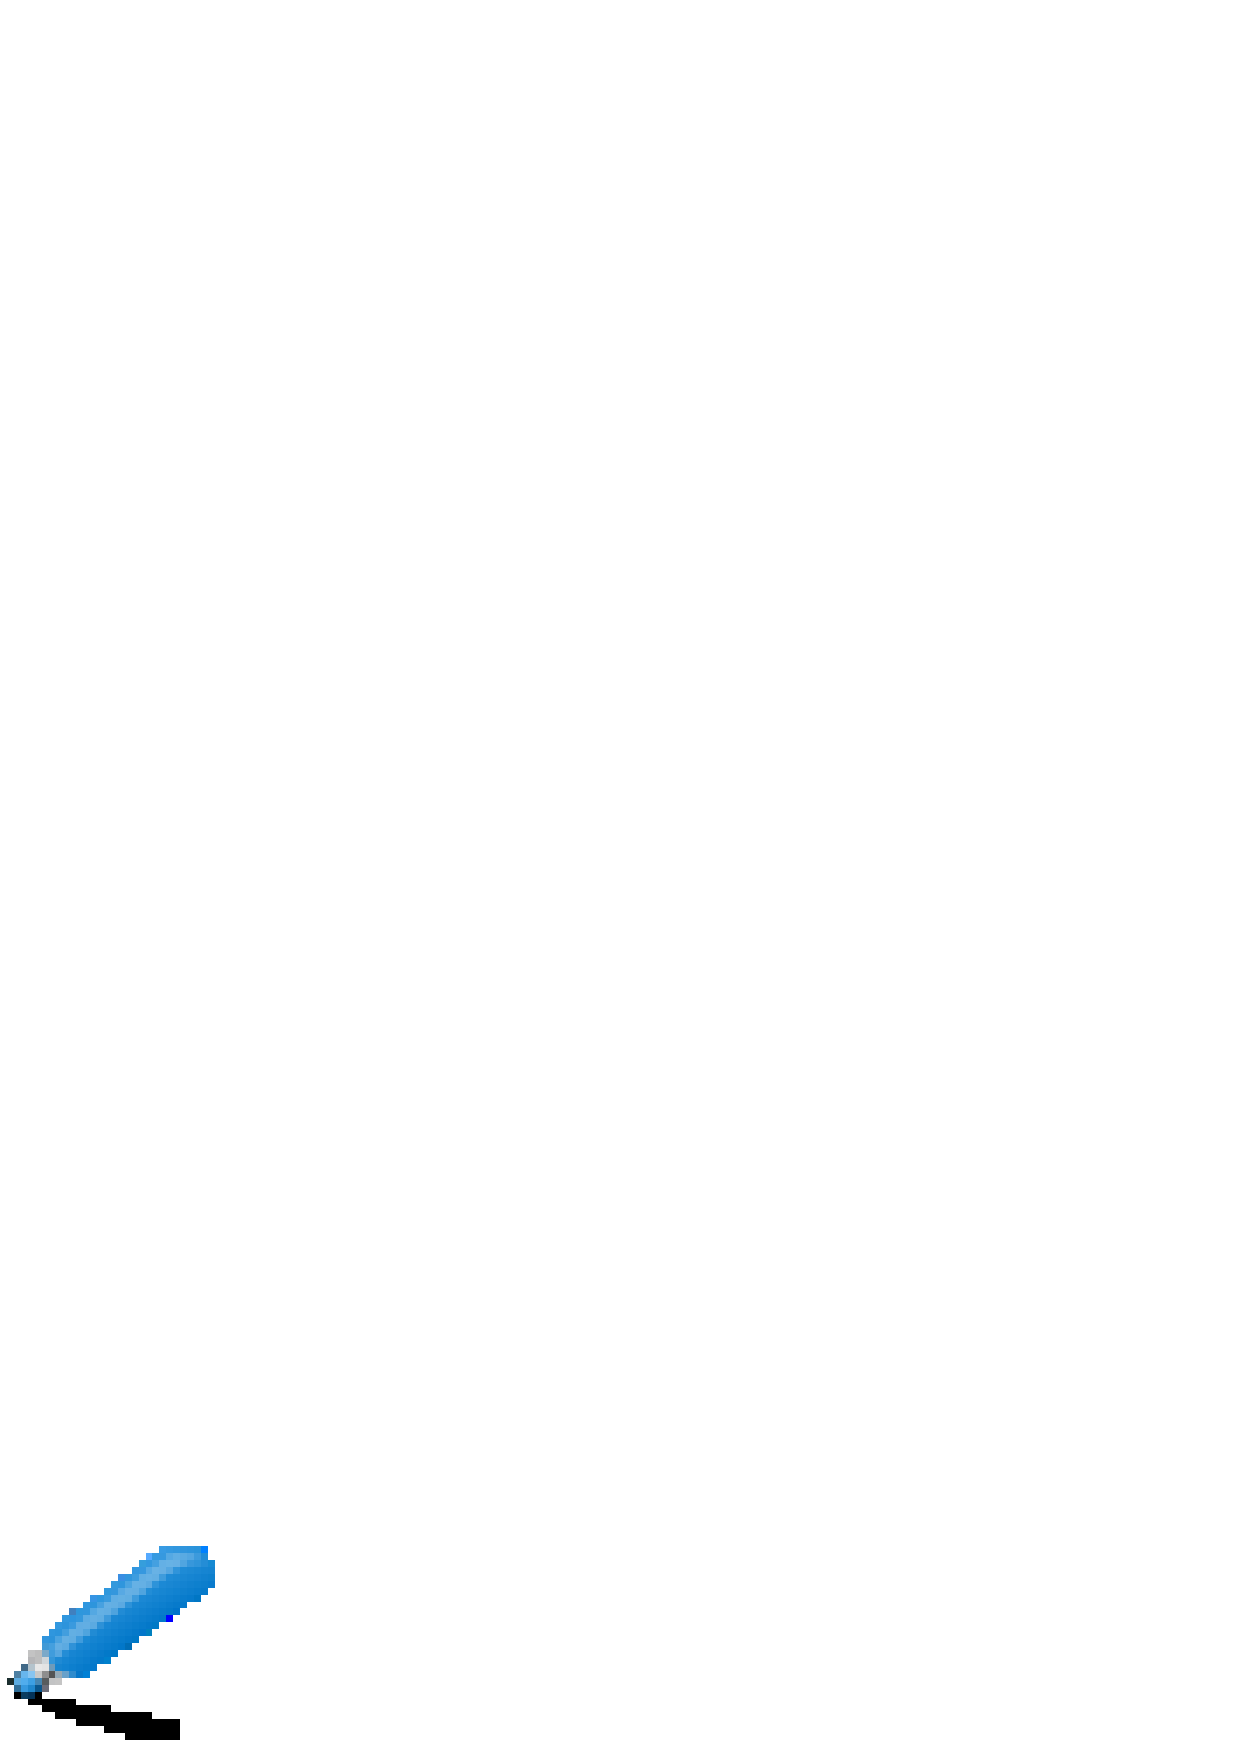
\includegraphics[width=0.7cm]{mActionToggleEditing}
   & Режим редактирования
   & 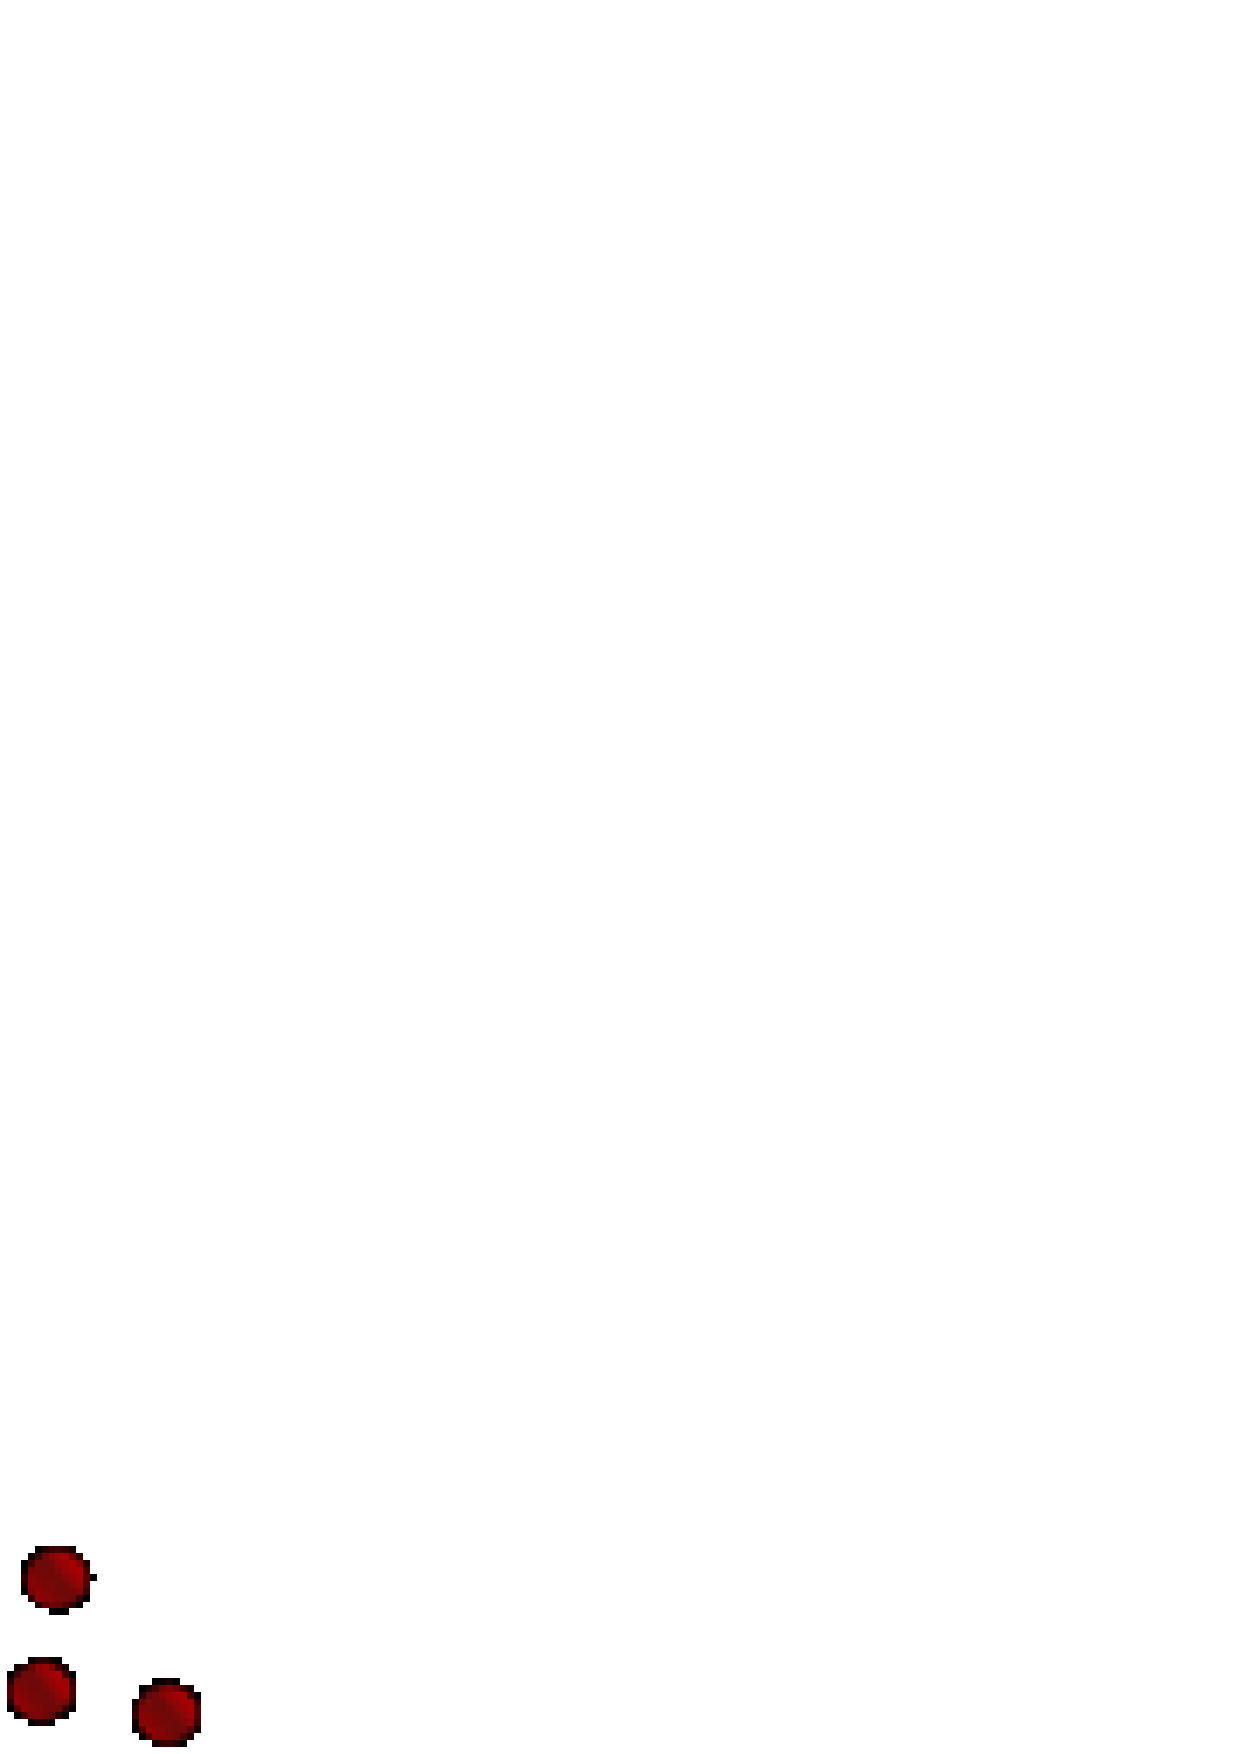
\includegraphics[width=0.7cm]{mActionCapturePoint}
   & Создать точку \\
\hline 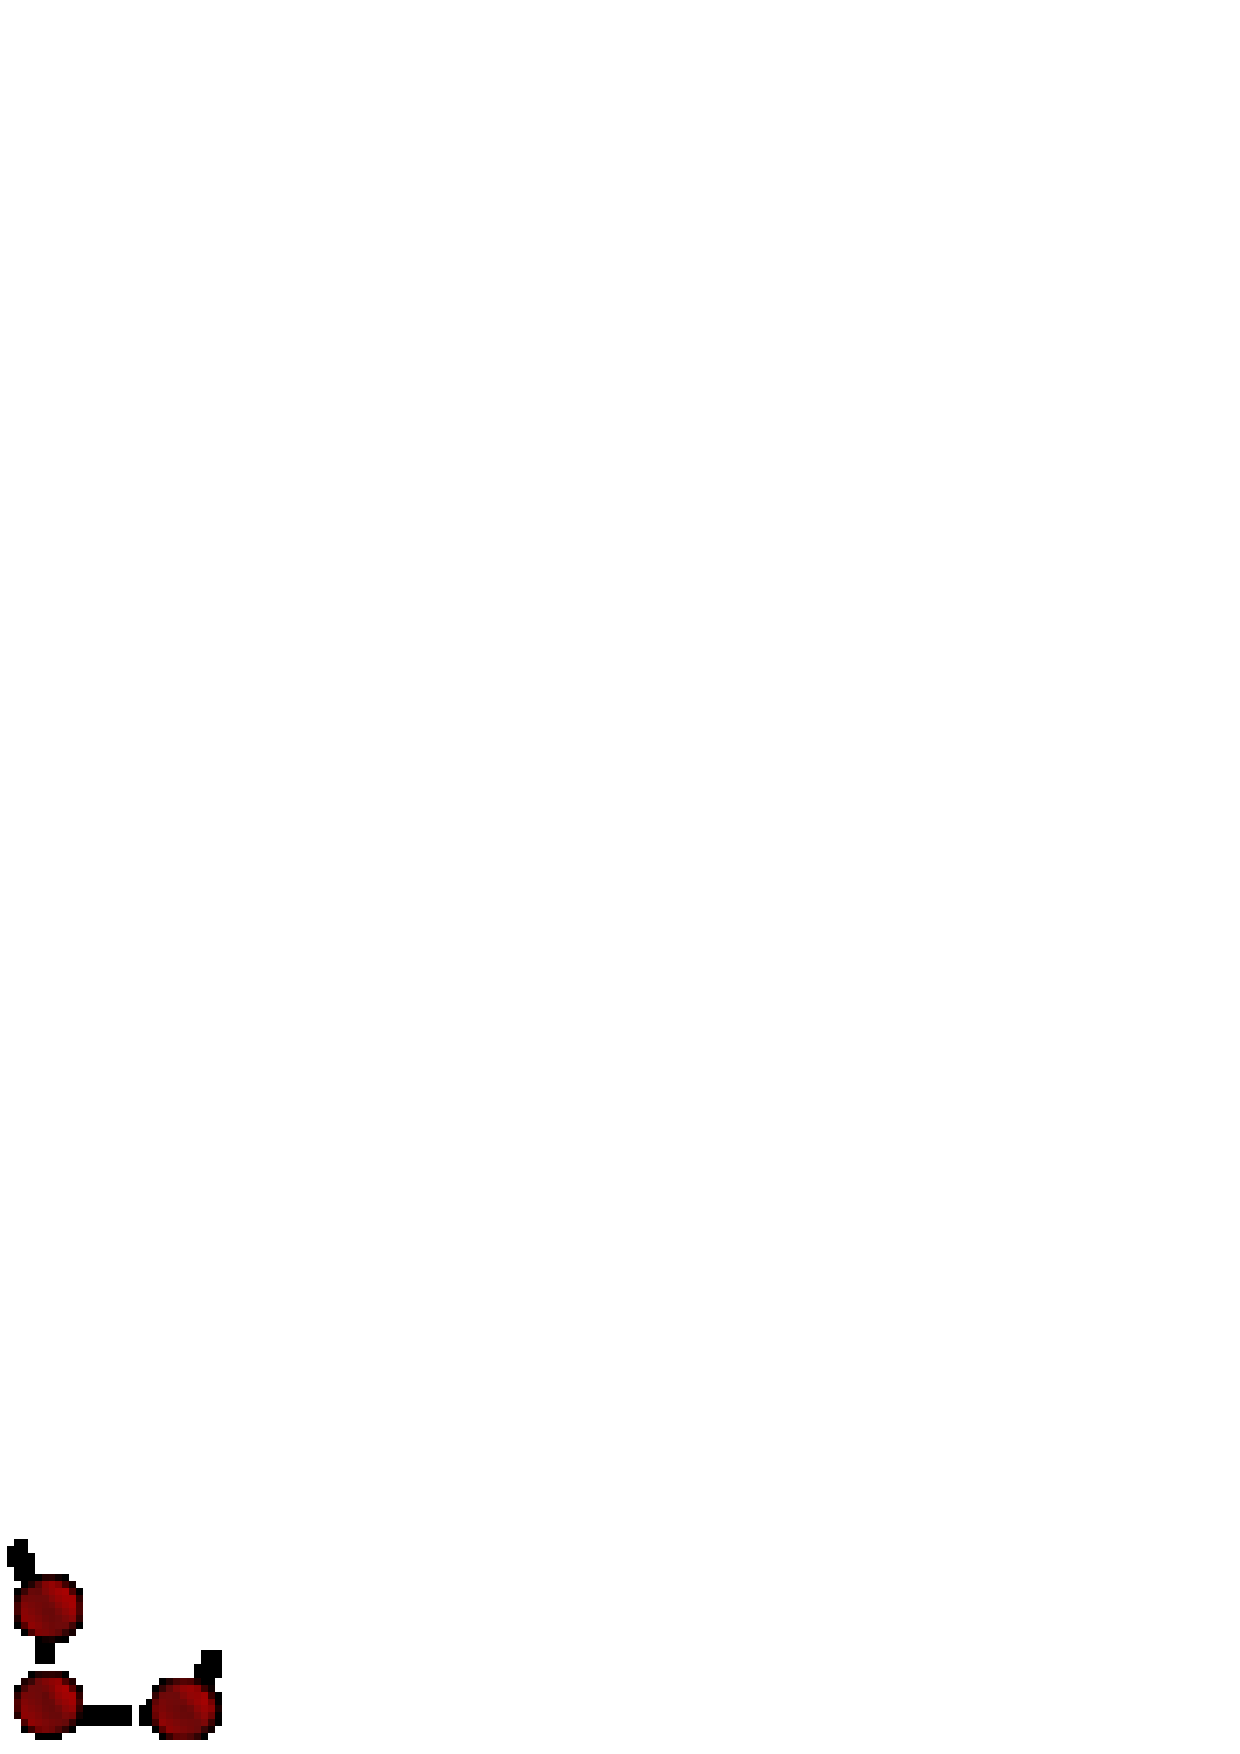
\includegraphics[width=0.7cm]{mActionCaptureLine}
   & Создать линию
   & 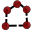
\includegraphics[width=0.7cm]{mActionCapturePolygon}
   & Создать полигон \\
\hline 
\includegraphics[width=0.7cm]{mActionMoveFeature}
   & Переместить объект
   & 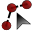
\includegraphics[width=0.7cm]{mActionNodeTool}
   & Редактирование узлов \\
\hline 
\includegraphics[width=0.7cm]{mActionDeleteSelected}
   & Удалить выделенное
   & 
\includegraphics[width=0.7cm]{mActionEditCut}
   & Вырезать объекты \\
\hline 
\includegraphics[width=0.7cm]{mActionEditCopy}
   & Копировать объекты
   & 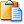
\includegraphics[width=0.7cm]{mActionEditPaste}
   & Вставить объекты \\
\hline 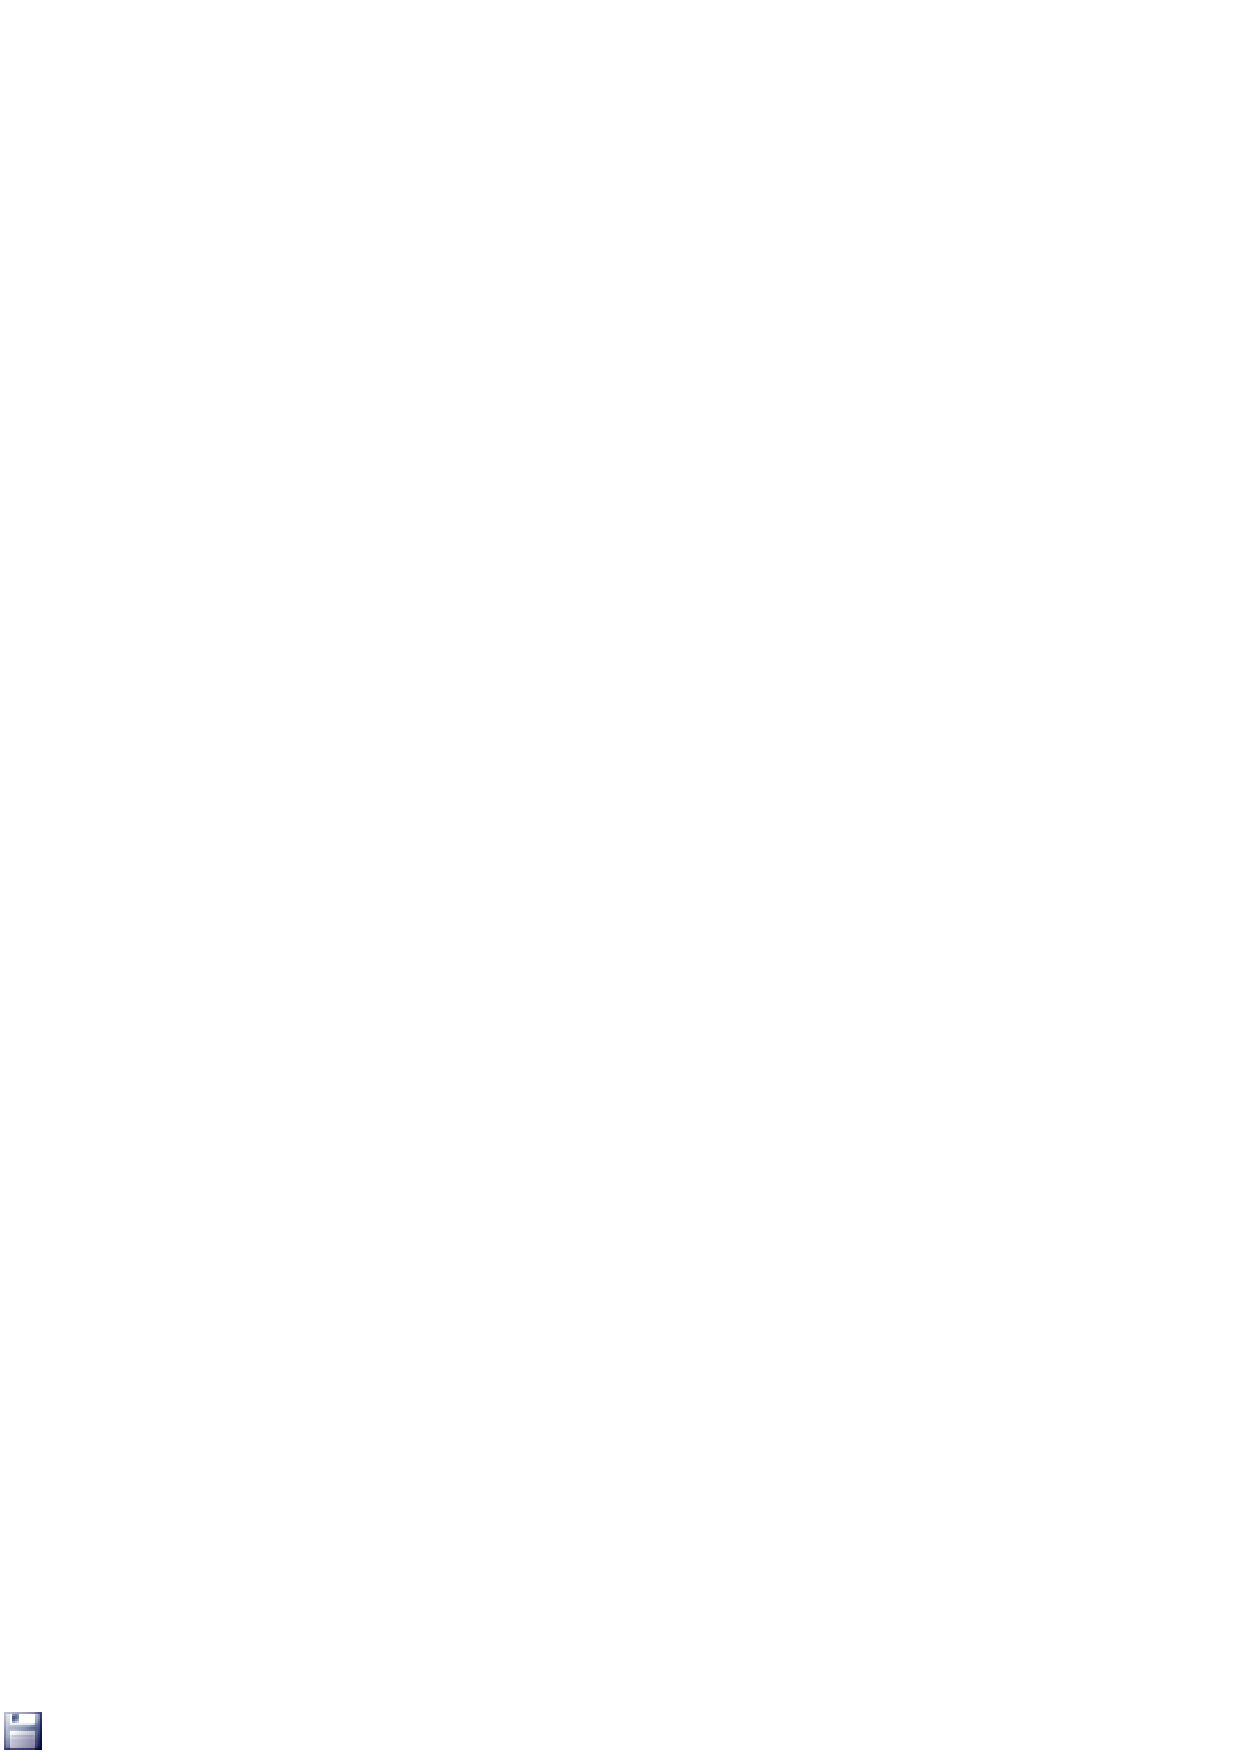
\includegraphics[width=0.7cm]{mActionFileSave}
   & Сохранить изменения
   &  &  \\
\hline
\end{tabular}
\caption{Основные инструменты редактирования векторного слоя}\label{tab:vector_editing}\medskip
\end{table}

Любое редактирование начинается с выбора функции
\dropmenuopttwo{mActionToggleEditing}{Режим редактирования}.
Эта опция доступна из контекстного меню после щелчка правой кнопки мыши
по легенде слоя.\index{режим редактирования}

Также, чтобы начать или закончить редактирование, можно использовать
кнопку \index{режим редактирования}
\toolbtntwo{mActionToggleEditing}{Режим редактирования} на панели инструментов
по оцифровке. После того, как слой стал редактируемым,
над каждой вершиной появятся специальные маркеры и станут доступными кнопки
с дополнительными функциями из панели инструментов.

\begin{Tip}\caption{\textsc{Регулярное сохранение}}
Не забывайте переключать \toolbtntwo{mActionToggleEditing}{Режим редактирования}
регулярно. Это позволит не только сохранить последние изменения, но и удостовериться,
что источники данных могут принять все сделанные изменения.
\end{Tip}

\minisec{Добавление объектов}
\index{векторные слои!добавление!объекта}
\index{векторные слои!перемещение!объекта}

Можно использовать кнопки на панели инструментов:
\toolbtntwo{mActionCapturePoint}{Создать точку},
\toolbtntwo{mActionCaptureLine}{Создать линию} или
\toolbtntwo{mActionCapturePolygon}{Создать полигон}, чтобы переключить \qg
в режим редактирования.

Для каждого объекта сначала идет оцифровка формы, а затем добавляются атрибуты.
Чтобы начать оцифровку и создать первую точку нового объекта, надо нажать
левой кнопкой мыши в области карты.

Для продолжения линий и полигонов надо продолжать нажимать на левую кнопку
мыши для создания каждого дополнительного узла. Чтобы закончить
редактирование объекта, просто щелкните правой кнопки мыши в любом
месте карты. Это подтверждение того, что редактирование данного объекта
окончено.

В процессе редактирования будет появляться окно атрибутов, позволяя тем
самым вводить информацию для нового объекта.
Рисунок~\ref{fig:vector_digitising} показывает ввод атрибутов для вымышленной реки
Аляски. В вкладке \tab{Оцифровка} из меню \mainmenuopt{Установки} \arrow
\dropmenuopt{Параметры} можно также активировать функцию \\
\checkbox{Не показывать всплывающее окно ввода атрибутов для каждого создаваемого объекта}.

\begin{figure}[ht]
   \centering
   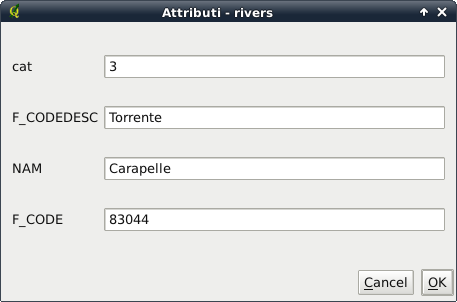
\includegraphics[clip=true, width=8cm]{editDigitizing}
   \caption{Диалог ввода атрибутивных значений после оцифровки нового объекта \wincaption}\label{fig:vector_digitising}
 \end{figure}

С помощью опции \toolbtntwo{mActionMoveFeature}{Переместить объект} на
панели инструментов можно двигать созданные объекты.

\begin{Tip}\caption{\textsc{Типы значений атрибутов}}
При редактировании shape-файла типы атрибутов проверяются во время ввода.
Поэтому невозможно ввести числовое значение в текстовое поле диалога
\dialog{Атрибуты} или наоборот. Если это сделать все же необходимо,
то следует отредактировать атрибуты на следующем шаге в диалоге
\dialog{Таблица атрибутов}.
\end{Tip}

\minisec{Редактирование узлов}
\index{векторные слои!узлы!инструмент}

Как для слоев данных PostgreSQL/PostGIS, так и для слоев, состоящих из
shape-файлов, \\
\toolbtntwo{mActionNodeTool}{Редактирование узлов} предоставляет
возможности изменения узлов объектов, аналогичные имеющимся в программах CAD.
Можно выделить сразу множество вершин и перемещать, добавлять или удалять
их все вместе. Инструмент редактирования узлов работает с включенной функцией
перепроецирования <<на лету>>, а также поддерживает топологическое редактирование
объектов. Этот инструмент, в отличие от остальных инструментов Quantum~GIS,
довольно <<настойчивый>>: так, когда некоторая операция выполнена, инструмент
продолжает оставаться активным, а объект выделенным. Если инструмент
редактирования узлов не может обнаружить объекты, на дисплей выдается
предупреждение.

Важно правильно установить \mainmenuopt{Установки} \arrow
\dropmenuopttwo{mActionOptions}{Параметры} \arrow
\tab{Оцифровка} \arrow \\ \selectnumber{{}Радиус поиска}{10}, значение должно быть
больше нуля. В противном случае \qg не распознает редактируемую вершину.

\begin{Tip}\caption{\textsc{Маркировка Вершин}}
Данная версия \qg поддерживает три типа маркировки вершин "--- полупрозрачный
круг, крест и <<без маркера>>. Чтобы изменить стиль маркировки, выберите
\dropmenuopttwo{mActionOptions}{Параметры} из меню \mainmenuopt{Установки}
и на вкладке \tab{Оцифровка} выберите подходящий тип.
\end{Tip}

\minisec{Основные операции}\index{векторные слои!редактирование узлов}

Включите инструмент \toolbtntwo{mActionNodeTool}{Редактирование узлов} и
выделите объект простым нажатием на него. На месте каждой вершины этого
объекта появятся красные рамки. Это основной инструмент выделения объектов.
Его функциональные возможности следующие:

\begin{itemize}[label=--]
\item \textbf{Выделение вершин}: Выделение узла происходит простым нажатием
по нему кнопкой мыши, при этом цвет рамки изменится на синий. Чтобы выделить
несколько узлов одновременно, надо удерживать клавишу
\keystroke{Shift}. Нажатие на
\keystroke{Ctrl} используется для инвертирования выделения узлов (выделенные
узлы становятся невыделенными и наоборот). Также несколько узлов одновременно
можно выделить, если нажать кнопкой мыши где-нибудь в стороне от объекта и
очертить прямоугольную область вокруг интересующего множества вершин. Или
просто нажать на отрезок линии и оба смежных узла будут выделены.
\item \textbf{Добавление узлов}: Добавить узлы также просто. Двойной щелчок
мыши рядом с отрезком линии добавит новую вершину рядом с положением курсора.
Обратите внимание, что вершина появится на ребре объекта, а не точно в
месте курсора,но при необходимости ее можно переместить.
\item \textbf{Удаление узлов}: После выделения вершин для их удаления надо
нажать клавишу \keystroke{Delete}, вершины будут удалены. Обратите внимание,
что, согласно стандарту Quantum~GIS, необходимое количество узлов для каждого
типа объекта все же останется. Чтобы полностью удалить объект, надо использовать
другой инструмент.
\item \textbf{Перемещение узлов}: Выделите все вершины, которые собираетесь
перемещать. Все выделенные вершины будут перенесены в направлении курсора.
Если активна функция прилипания, все вершины могут перескочить на
ближайшие узлы или линии.
\end{itemize}

При отпускании кнопки мыши все изменения будут сохранены и появятся в
диалоге отмены. Запомните, что все операции поддерживают топологическое
редактирование, когда оно включено. Перепроецирование <<на лету>> также
поддерживается.

\minisec{Вырезать, копировать и вставить объекты}
\index{векторные слои!вырезать!объект}
\index{векторные слои!копировать!объект}
\index{векторные слои!вставить!объект}
\index{редактирование!вырезание объектов}
\index{редактирование!копирование объектов}
\index{редактирование!вставка объектов}

Выделенные объекты можно удалять, копировать и вставлять из слоя в слой
одного проекта \qg  при условии, что для них включен
\toolbtntwo{mActionToggleEditing}{Режим редактирования}.

Объекты также можно вставить во внешние приложения в виде текста: объекты
отражаются в формате  CSV, где их геометрия передается форматом
OGC Well-Known Text (WKT).

Однако в настоящей версии  \qg текстовые объекты из внешних приложений
\qg не могут быть добавлены в слой \qg. Когда же может пригодиться функция
копирования и вставки? Оказывается, возможно редактирование нескольких
слоев одновременно и копирование/вставка объектов между ними. Для чего это
может понадобиться? Предположим, необходимо поработать со слоем озер, в
котором интересует только одно или два озера, а не все 5\,000, как, например,
в нашем слое \filename{big\_lakes}. Тогда можно создать новый слой и,
используя операции копирование/вставка, переместить в него нужные озера.

Рассмотрим пример копирования отдельных озер в новый слой:

\begin{enumerate}
\item Загрузить слой, из которого вы собираетесь копировать (исходный слой)
\item Загрузить или создать слой, в который вы будете копировать (целевой слой)
\item Начать редактирование целевого слоя
\item Активировать исходный слой щелчком мыши по нему в легенде
\item Используя инструмент \toolbtntwo{mActionSelect}{Выбрать объекты},
выделить объект(ы) в исходном слое
\item Выбрать инструмент \toolbtntwo{mActionEditCopy}{Копировать объекты}
\item Сделать активным целевой слой, щелкнув по нему в легенде кнопкой мыши
\item Нажать \toolbtntwo{mActionEditPaste}{Вставить выделенные объекты}
\item Завершить редактирование и сохранить изменения
\end{enumerate}

Что случится, если исходный и целевой слой имеют разную структуру (названия
полей и их типы отличаются)? \qg заполнит совпадающие поля и проигнорирует
остальные. Если результат копирования атрибутов в целевой слой не имеет
значения, то становится неважно, в каком виде они там будут представлены.
Если в целевом слое необходимо сохранить все с точностью "--- объекты и
их атрибуты, необходимо убедиться, что структуры исходного и целевого слоя
совпадают.

\begin{Tip}\caption{\textsc{Соответствие вставляемых объектов}}
Если исходный и целевой слой находятся в одинаковой проекции, тогда
геометрия вставленных объектов будет идентична исходному слою. Однако если
целевой слой находится в проекции, отличной от исходной, тогда \qg не гарантирует
идентичность геометрии. Это происходит по причине незначительных ошибок
округления, неизбежных при переходе от одной проекции к другой.
\end{Tip}

\minisec{Удаление выделенных объектов}
\index{векторные слои!удаление!объекта}

Если надо удалить весь полигон, вначале его необходимо выделить, используя
обычный инструмент \\
\toolbtntwo{mActionSelect}{Выбрать объекты}. Также можно
выделить несколько объектов для удаления. После выбора соответствующих
объектов используйте инструмент
\toolbtntwo{mActionDeleteSelected}{Удалить выделенное}, объекты будут удалены.

Инструмент \toolbtntwo{mActionEditCut}{Вырезать выделенные объекты} на панели
инструментов по оцифровке также может использоваться для удаления объектов.
Это действительно удаляет объекты, но также помещает их в <<пространственный
буфер>>. Таким образом, вырезание объектов приводит к их удалению. Затем можно
использовать инструмент \toolbtntwo{mActionEditPaste}{Вставить выделенные объекты},
чтобы вернуть их обратно. Это дает возможность отменить выполненное удаление
объекта. Операции вырезания, копирования и вставки работают только на
выделенных объектах, это означает, что можно работать с несколькими объектами
одновременно.

\begin{Tip}\caption{\textsc{Поддержка удаления объектов}}
Когда редактируется shape-файл, удаление объектов из него возможно, если
\qg использует версию GDAL 1.3.2 или выше. Версии \qg для операционных
систем OS\,X и Windows, доступные для скачивания на официальном сайте,
сделаны с использованием версии GDAL 1.3.2 или выше.
\end{Tip}

\minisec{Сохранение отредактированных слоев}
\index{редактирование!сохранение}

Когда слой находится в режиме редактирования, любые изменения сохраняются
только в памяти \qg. Поэтому они не сохраняются непосредственно на диск.
Если необходимо сохранить изменения в текущем слое и при этом продолжать
его редактирование, нужно просто нажать на кнопку
\toolbtntwo{mActionFileSave}{Сохранить изменения}. Если выключить режим
редактирования нажав на \toolbtntwo{mActionToggleEditing}{Режим редактирования}
(или просто выйти из \qg), то появится запрос, хотите вы сохранить
изменения или нет.

Если изменения не могут быть сохранены (например, диск полон или атрибуты
имеют неверное значение), \qg сохранит их в своей памяти. Это позволит
откорректировать изменения и попробовать еще раз.

\begin{Tip}\caption{\textsc{Целостность данных}}
Создание резервной копии данных перед началом редактирования "--- это
всегда хорошая идея. Несмотря на то, что авторы \qg сделали все возможное
для сохранения ваших данных, они по-прежнему не дают никаких гарантий в
этом отношении.
\end{Tip}

\subsection{Дополнительные функции оцифровки}
\index{векторные слои!дополнительные функции оцифровки}
\index{дополнительные функции оцифровки!существующего слоя}
\label{sec:advanced_edit}

\begin{table}[h]\index{векторные слои!дополнительные инструменты редактирования}
\centering
\small
\begin{tabular}{|l|p{6.9cm}|l|p{6.9cm}|}
\hline \textbf{Иконка} & \textbf{Назначение} & \textbf{Иконка} & \textbf{Назначение} \\
\hline 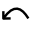
\includegraphics[width=0.7cm]{mActionUndo}
   & Отменить
   & 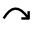
\includegraphics[width=0.7cm]{mActionRedo}
   & Вернуть \\
\hline \includegraphics[width=0.7cm]{mActionSimplify}
   & Упростить объект
   & \includegraphics[width=0.7cm]{mActionAddRing}
   & Добавить кольцо \\
\hline \includegraphics[width=0.7cm]{mActionAddIsland}
   & Добавить часть
   & \includegraphics[width=0.7cm]{mActionDeleteRing}
   & Удалить кольцо \\
\hline \includegraphics[width=0.7cm]{mActionDeletePart}
   & Удалить часть
   & \includegraphics[width=0.7cm]{mActionReshape}
   & Корректировать объекты \\
\hline \includegraphics[width=0.7cm]{mActionSplitFeatures}
   & Разбить объекты
   & \includegraphics[width=0.7cm]{mActionMergeFeatures}
   & Объединить выбранные объекты \\
\hline \includegraphics[width=0.7cm]{mActionRotatePointSymbols}
   & Повернуть значки
   &
   & \\
\hline
\end{tabular}
\caption{Дополнительные возможности редактирования векторного слоя}\label{tab:advanced_editing}
\end{table}

\minisec{Отменить и Вернуть}
\index{векторные слои!отменить}
\index{векторные слои!вернуть}

Инструменты \toolbtntwo{mActionUndo}{Отменить} и
\toolbtntwo{mActionRedo}{Вернуть} позволяют отменить либо вернуть
последний или какой-либо конкретный шаг при редактировании векторных данных.
Основной вид операций Отменить/Вернуть представляет из себя виджет, где
показаны все действия (см. Рисунок~\ref{fig:vector_redoundo}). Этот виджет
по умолчанию не показывается, чтобы он появился, надо нажать правой кнопкой
мыши по панели инструментов и кликнуть по флажку Отменить/Вернуть. Однако
функция Отменить/Вернуть активна, даже если виджет не выведен на экран.

При нажатии кнопки \button{Отменить} состояние всех объектов и их атрибутов
возвращается на шаг назад. Изменения, произведенные в каком-либо другом
месте (например, в одном из модулей), могут иметь неспецифические названия
для своих операций, которые появляются в этой закладке. Операции можно
отменить или оставить их изменения.

Действия можно отменить простым нажатием на кнопки \button{Отменить} или
\button{Вернуть}, либо выбрать непосредствено на пункт из списка, который
хотите отменить. Другая возможность отменить операцию "--- нажать на кнопку
\button{Отменить/Вернуть} на панели инструментов дополнительных возможностей
редактирования.

\begin{figure}[ht]
   \centering
   \includegraphics[clip=true, width=12cm]{redo_undo}
   \caption{Отмена и Возврат операций редактирования \wincaption}\label{fig:vector_redoundo}
\end{figure}

\minisec{Упростить объект}
\index{векторные слои!упростить}

Инструмент \toolbtntwo{mActionSimplify}{Упростить объект} позволяет уменьшить
количество вершин объекта, при этом, геометрия объекта не изменяется.
Необходимо выделить объект, после чего он будет подсвечен красным и появится
ползунок. При движении ползунка красная опоясывающая линия меняет свою форму,
показывая тем самым, как именно объект будет упрощен. Если нажать кнопку \button{OK},
новая упрощенная геометрия будет сохранена. Если объект не может быть
упрощен (например, мультиполигоны), появится всплывающее окно предупреждения.

\minisec{Добавить кольцо}
\index{векторные слои!добавить!кольцо}

Можно создать кольцевой полигон, используя функцию
\toolbtntwo{mActionAddRing}{Добавить кольцо} на панели инструментов. Внутри
существующего полигона можно оцифровать последующий полигон, который
превратиться в <<отверстие>>, таким образом, только оставшаяся область
между границами внешнего и внутреннего полигона и будет кольцевым полигоном.

\minisec{Добавить часть}
\index{векторные слои!добавить!часть}

Можно использовать \toolbtntwo{mActionAddIsland}{Добавить часть}
для добавления новых полигонов к мультиполигональным объектам. Новая
полигональная часть должна быть создана за границами мультиполигона.


\minisec{Удалить кольцо}
\index{векторные слои!удалить!кольцо}

Инструмент \toolbtntwo{mActionDeleteRing}{Удалить кольцо} позволяет удалять
кольцевые полигоны внутри существующей площади. Этот инструмент работает
только с полигональными слоями. Никакик изменений не произойдет, если
инструмент применяется на внешнем контуре полигона. Инструмент может
применяться как для полигональных объектов, так и на мультиполигональных.
Перед тем, как выделить вершины кольца, настройте порог прилипания для вершин.


\minisec{Удалить часть}
\index{векторные слои!удалить!часть}

Инструмент \toolbtntwo{mActionDeletePart}{Удалить часть} позволяет удалять
части мультиполигональных объектов (например, удалить полигон
мультиполигонального объекта). Инструмент не сможет удалить последнюю часть
объекта. Она останется нетронутой. Инструмент работает со всеми типами
геометрии: точками, линиями, полигонами. Перед тем, как выделить вершины
части, необходимо настроить порог прилипания для вершин.

\minisec{Корректировать объекты}
\index{векторные слои!корректировать!объект}

Можно корректировать форму линий и полигонов, используя инструмент
\toolbtntwo{mActionReshape}{Корректировать объекты}, расположенный на
панели инструментов. Он удаляет часть линии или полигона между первым и
последним пересечением с исходной линией. При работе с полигонами это
может иногда привести к непредсказуемым результатам. Этот инструмент
наиболее пригоден для корректировки небольших частей полигонов. Редактирование
нескольких  полигональных объектов одновременно невозможно, так как при этом
будут создаваться полигоны с ошибочной геометрией.

\textbf{Примечание}: Инструмент корректировки объектов может изменять начало
кольца полигона или замкнутой линии. Так, точка, представленная «дважды»,
больше не будет таковой. Это не должно быть проблемой при использовании
большинства приложений, но, тем не менее, это необходимо иметь в виду.

\minisec{Разбивка объектов}
\index{векторные слои!разбить!объект}

Можно разбить объекты, используя инструмент
\toolbtntwo{mActionSplitFeatures}{Разбить объекты} на панели
инструментов. Чтобы разбить объект, просто нарисуйте линию через него.

\minisec{Объединить выделенные объекты}
\index{векторные слои!объединить!объекты}

Инструмент \toolbtntwo{mActionMergeFeatures}{объединить выделенные объекты}
позволяет объединять объекты, которые имеют общие границы и атрибуты.

\minisec{Повернуть значки}
\index{векторные слои!повернуть!значок}

Инструмент \toolbtntwo{mActionRotatePointSymbols}{Повернуть значки} позволяет
изменить поворот точечного символа на карте, если задано вращение по столбцу
атрибутивной таблицы точечного слоя на вкладке \tab{Символика} из меню
свойств слоя "--- \dialog{Свойства}. В другом случае инструмент будет
неактивным.

\begin{figure}[ht]
   \centering
   \includegraphics[clip=true, width=6cm]{rotatepointsymbol}
   \caption{Поворот точечного символа \wincaption}\label{fig:rotatepoint}
\end{figure}

Чтобы повернуть объект, выделите точечный объект на карте и вращайте его,
удерживая нажатой левую кнопку мыши. При этом будет отображаться красная
стрелка с величиной угла поворота (см. Рисунок~\ref{fig:rotatepoint}).
Когда вы отпустите левую кнопку мыши, в таблице атрибутов обновится значение.

\textbf{Примечание}: Если удерживать кнопку \keystroke{Ctrl} нажатой, поворот
будет осуществляться с шагом 15 градусов.

\subsection{Создание новых слоёв в формате shape-файл и Spatialite}\label{sec:create shape}\index{редактирование!создание нового слоя}

\qg позволяет создавать новые shape-файлы и слои Spatialite. Создание новых
слоев GRASS осуществляется с помощью расширения GRASS. Для более подробной
информации по созданию слоев GRASS обратитесь к Разделу~\ref{sec:creating_new_grass_vectors}.

\minisec{Создание нового shape-файла}\label{sec:create shape}\index{редактирование!создание нового shape-файла}

Чтобы создать новый редактируемый shape-файл, выберите \button{Создать} \arrow
\toolbtntwo{mActionNewVectorLayer}{Создать новый shape-файл} из меню
\mainmenuopt{Слой}. Появится диалог \dialog{Новый векторный слой}, как показано
на Рисунке~\ref{fig:newvectorlayer}. Выберите тип слоя (точка, линия или полигон).

\begin{figure}[ht]
   \centering
   \includegraphics[clip=true, width=8cm]{editNewVector}
   \caption{Диалог создания нового shape-файла \wincaption}\label{fig:newvectorlayer}
\end{figure}

Обратите внимание, что \qg пока еще не поддерживает создание объектов в
размерности 2.5D (т.\,е. объектов с координатами X, Y, Z), кроме того, не
поддерживается создание объектов с линейной системой координат (координата M).
В настоящее время можно создавать только shape-файлы. В будущих
версиях \qg будет поддерживаться создание любых слоев типов OGR или PostgreSQL.

В завершении создания shape-файла следует добавить желаемые атрибуты. Для
этого надо нажать на кнопку  \button{Добавить} и задать имя и тип атрибутов.
Поддерживаются только следующие типы атрибутов:  \selectstring{{}Тип}{Текст},
\selectstring{{}Тип}{Целое число}, и \selectstring{{}Тип}{Десятичное число}.
Дополнительно, в соответствии с выбранным типом атрибута, можно определить
размер и точность для нового поля атрибутов. Как только все необходимые
параметры заданы, нажмите кнопку \button{OK} и задайте имя для выходного
shape-файла. \qg автоматически добавит к имени файла расширение \filename{.shp}.
После того, как shape-файл создан, он будет добавлен в карту и доступен для
обычного редактирования, как описано в Разделе~\ref{sec:edit_existing_layer} выше.

\minisec{Создание нового слоя SpatiaLite}\label{sec:create spatialite}\index{редактирование!создание нового слоя SpatiaLite}

Чтобы создать новый редактируемый слой SpatiaLite, выберите \button{Создать}
\arrow \toolbtntwo{mActionNewVectorLayer}{Создать слой SpatiaLite} из меню
\mainmenuopt{Слой}. Появится диалог \dialog{Создать слой SpatiaLite}, как
показано на Рисунке~\ref{fig:newspatialitelayer}.

\begin{figure}[ht]
   \centering
   \includegraphics[clip=true, width=8cm]{editNewSpatialite}
   \caption{Диалоговое окно <<Создать слой SpatiaLite>> \wincaption}\label{fig:newspatialitelayer}
\end{figure}

Первый шаг "--- выбрать существующую базу данных SpatiaLite или создать
новую. Загрузить существующую базу данных можно, нажав на кнопку \button{...}
справа от поля имени для базы данных. Затем следует задать имя новому слою и
определить тип слоя и EPSG SRID. По желанию можно выбрать \\
\checkbox{создать первичный ключ с автоматическим приращением}.

Чтобы задать таблицу атрибутов для нового слоя SpatiaLite, добавьте имена
и определите соответствующие типы данных для новых столбцов таблицы, затем
нажмите кнопку \button{Добавить}. В завершение нажмите кнопку \button{OK}.
\qg автоматически добавит новый слой в легенду, и он будет доступен для
обычного редактирования, как описано в Разделе~\ref{sec:edit_existing_layer} выше.

В диалоговом окне создания слоя SpatiaLite можно создать несколько слоев,
нажимая на кнопку \button{Apply}, при этом нет необходимости закрывать
диалоговое окно.

\subsection{Работа с таблицей атрибутов}
\label{sec:attribute table}
\index{редактирование!работа с таблицей атрибутов}

Таблица атрибутов представляет объекты выделенного слоя. Каждая строка таблицы
соответствует одному объекту на карте и отражает его атрибуты в столбцах.
Объекты в таблице можно искать, выделять, перемещать и редактировать.

Чтобы открыть таблицу атрибутов векторного слоя, необходимо сделать его активным,
нажав по нему кнопкой мыши в легенде карты. Затем в меню \mainmenuopt{Слой}
выберите \dropmenuopttwo{mActionOpenTable}{Открыть таблицу атрибутов}.
Также можно открыть таблицу атрибутов, щелкнув по слою в легенде правой
кнопкой мыши, и выбрав \\
\dropmenuopttwo{mActionOpenTable}{Открыть таблицу атрибутов}
из выпадающего меню. Откроется новое окно, в котором будут представлены атрибуты
для каждого объекта слоя (cм. Рисунок~\ref{fig:attributetable}). Количество
объектов указано в заголовке атрибутивной таблицы.

\begin{figure}[ht]
   \centering
   \includegraphics[clip=true, width=12cm]{vectorAttributeTable}
   \caption{Таблица атрибутов слоя Alaska \wincaption}\label{fig:attributetable}
\end{figure}

\minisec{Выделение объектов по таблице атрибутов}

\textbf{Выделенная строка} в таблице атрибутов представляет все атрибуты
выделенного объекта слоя. Таблица атрибутов отражает все изменения в
выделении объектов слоя через главное окно карты или наоборот. Смена
выделения в таблице атрибутов приводит к изменению выделения в главном
окне карты, также выделение другого объекта слоя приводит к выделению
соответствующей ему строки таблицы.

Строки можно выделить, если нажать кнопкой мыши на номер строки, расположенный
слева от неё. Выделение строки не меняет текущего положения курсора.
\textbf{Несколько строк} можно выделить, удерживая клавишу \keystroke{Ctrl}.
Также доступно \textbf{Сквозное выделение}, для этого необходимо
удерживать клавишу \keystroke{Shift} и выбрать несколько строк, также
нажимая на их номера-заголовки, расположенные слева. Все строки между
текущим положением курсора и выбранными строками будут выделены.

Каждый столбец может быть отсортирован. Для этого надо нажать кнопкой мыши
на его заголовоке. Небольшая стрелка отражает порядок сортировки (направленная
вниз стрелка означает убывание величины от верхних строк к нижним, а
направленная вверх стрелка означает возрастание величины от верхних строк
к нижним).

Для \textbf{простого поиска по атрибутам} только по одному столбцу можно
использовать поле \button{Искать?}. Выберите поле (столбец), по которому
хотите произвести поиск, из выпадающего меню, и нажмите кнопку \\ \button{Поиск}.
Количество сопоставленных записей появится в окне результатов. Для более
сложного поиска используйте Расширенный поиск \button{...}, который будет
описан в Разделе~\ref{sec:select_by_query}.

Чтобы отобразить только выбранные строки, нажмите кнопкой мыши в окошке \\
\checkbox{Показать только выбранные записи}. Для поиска только по выделенным
записям активируйте \\
\checkbox{Искать только в выбранных записях}. Остальные
кнопки, расположенные слева снизу атрибутивной таблицы, обладают следующими
функциями:

\begin{itemize}[label=--]
\item \toolbtntwo{mActionOpenTable}{Снять выделение}
\item \toolbtntwo{mActionSelectedToTop}{Переместить выделенные в начало}
\item \toolbtntwo{mActionInvertSelection}{Обратить выделение}
\item \toolbtntwo{mActionCopySelected}{Копировать выбранные строки в буфер обмена}
также с \keystroke{Ctrl-C}
\item \toolbtntwo{mActionZoomToSelected}{Увеличить карту до выбранных строк}
также с \keystroke{Ctrl-J}
\item \toolbtntwo{mActionToggleEditing}{Режим редактирования} для
редактирования отдельных значений таблицы атрибутов и активации функций,
описанных ниже.
\item \toolbtntwo{mActionDeleteSelected}{Удалить выделенные объекты}
\item \toolbtntwo{mActionNewAttribute}{Добавить поле} для слоев PostGIS
и OGR с версией GDAL >= 1.6.
\item \toolbtntwo{mActionDeleteAttribute}{Удалить поле} пока только для
слоев PostGIS.
\item \toolbtntwo{mActionCalculateField}{Открыть калькулятор полей}
\end{itemize}

\begin{Tip}\caption{\textsc{Управление атрибутивными данными}}
В настоящее время только для слоев PostGIS поддерживается добавление или
удаление столбцов атрибутов с помощью этого диалогового окна. В
будущих версиях \qg будут поддерживаться и другие источники данных,
так как это нововведение было недавно добавлено в GDAL/OGR > 1.6.0
\end{Tip}

\section{Конструктор поисковых запросов}\label{sec:query_builder}
\index{конструктор поисковых запросов}

Кнопка \button{Расширенный поиск\dots} открывает <<Конструктор поисковых
запросов>> и позволяет задать подмножество таблицы при помощи
<<SQL-условия WHERE>>, отображать результаты в главном окне и сохранять
их в качестве shape-файлов. Например, имеется слой \filename{towns}.
Используя поле \usertext{population}, можно выбрать только крупные города,
введя \usertext{population > 100000} в поле SQL-запроса <<Конструктора
поисковых запросов>>. Рисунок~\ref{fig:query_builder} демонстрирует пример
<<Конструктора поисковых запросов>>, заполненного данными из слоя PostGIS,
атрибуты которого хранятся в PostgreSQL. Секции <<Поля>>, <<Значения>>,
<<Операторы>> облегчают пользователю задание SQL-условия WHERE в
соответствующем поле.

\begin{figure}[ht]
  \centering
    \includegraphics[clip=true, width=11.5cm]{queryBuilder}
    \caption{Конструктор запросов \wincaption}\label{fig:query_builder}
\end{figure}

Список \textbf{Поля} содержит все атрибуты таблицы атрибутов. Для того,
чтобы добавить атрибут в поле SQL-условия, сделайте двойной щелчок мышью
по его имени из списка <<Поля>>. Можно использовать различные поля, значения
и операторы для составления запроса, а можно просто напечатать его в поле
SQL-условия.

Список \textbf{Значения} содержит значения атрибутов. Чтобы просмотреть все
значения атрибута, выберите нужный атрибут в списке <<Поля>> и нажмите кнопку
\button{Все} \index{конструктор поисковых запросов!получить все значения}. Нажатие кнопки
\button{Образец} после выбора нужного атрибута в списке <<Поля>> выводит
до 25 значений данного атрибута \index{конструктор поисковых запросов!получить пример значений}.
Чтобы добавить добавить конкретное значение в поле <<SQL-условия WHERE>>,
следует дважды щёлкнуть по нему в списке <<Значения>>.

Секция \textbf{Операторы} содержит все допустимые операторы. Чтобы добавить
оператор в поле <<SQL-условия WHERE>>, нажмите нужную кнопку. Доступны:
операторы отношения ( = , > , \ldots), оператор сравнения строк (LIKE),
логические операторы (AND, OR, \ldots).

Кнопка \button{Очистить} очищает поле <<SQL-условия WHERE>>. Нажатие кнопки
\button{Проверить} показывает окно сообщения с количеством записей,
удовлетворяющих данному запросу, что бывает очень полезно в процессе
построения запроса. Кнопка \button{OK} закрывает окно <<Конструктора
запросов>> и выбирает записи, удовлетворяющие запросу. Кнопка
\button{Отменить} закрывает окно, при этом текущая выборка остаётся
неизменной.

\begin{Tip}\caption{\textsc{Ограничение слоя}}\index{конструктор поисковых запросов!ограничение слоя}
При помощи SQL-запроса можно задать ограничение слоя. Для этого откройте
диалог \dialog{Свойства слоя} двойным щелчком по имени векторного слоя,
и нажмите на кнопку \button{Конструктор запросов} во вкладке \tab{Общие}.
Дополнительную информацию можно найти в Разделе~\ref{sec:vectorprops}
\end{Tip}

\minisec{Выделение при помощи запроса}\label{sec:select_by_query}

В \qg возможно осуществлять выборку, используя тот же интерфейс,
который описан в Разделе~\ref{sec:query_builder}. Выше демонстрировалось
использование <<Конструктора поисковых запросов>> только в целях отображения
записей, удовлетворяющих определённому критерию в качестве подмножества
<<виртуального слоя>> Цель выбора с помощью функции запроса заключается
в выделении всех записей, удовлетворяющих определённым условиям. Выделение
с помощью запроса может осуществляться с любым поддерживаемым форматом
векторных данных.

Чтобы осуществить операцию выделения при помощи запроса на загруженном слое,
нажмите кнопку \\
\toolbtntwo{mActionOpenTable}{Открыть таблицу атрибутов}, чтобы открыть
соответствующий диалог. Затем нажмите кнопку \
\button{Расширенный поиск} внизу, справа. Откроется <<Конструктор поисковых
запросов>>, который позволит задать подмножество данной таблицы и отобразить
его также, как описано в Разделе~\ref{sec:query_builder}.

\section{Калькулятор полей}\label{sec:field_calculator}
\index{PostgreSQL!калькулятор полей}
\index{PostGIS!калькулятор полей}
\index{OGR!калькулятор полей}
\index{калькулятор полей!PostgreSQL}
\index{калькулятор полей!PostGIS}
\index{калькулятор полей!OGR}

Кнопка \toolbtntwo{mActionCalculateField}{Калькулятор полей} в
таблице атрибутов позволяет осуществлять расчёты на основе существующих
значений атрибутов или заданных функций, например для расчёта длины или
площади геометрических объектов. Результаты могут быть записаны в новую
колонку атрибутов или использоваться для обновления значений существующей
колонки. Создание новых атрибутивных полей в данный момент возможно только
в PostGIS и в OGR-совместимых форматах, если версия GDAL >= 1.6.0.

Прежде чем нажать иконку <<Калькулятора полей>> (см. Рисунок~\ref{fig:field_calculator}),
необходимо перевести слой в режим редактирования. В появившемся диалоговом
окне сначала необходимо выбрать одну из опций: <<Обновить существующее поле>>,
<<Обновить только выбранные объекты>> или создать <<Новое поле>> таблицы
атрибутов, куда будут добавлены результаты вычислений.

\begin{figure}[ht]
  \centering
    \includegraphics[clip=true, width=11.5cm]{fieldcalculator}
    \caption{Калькулятор полей \wincaption}\label{fig:field_calculator}
\end{figure}

Чтобы добавить новое поле, необходимо указать его имя, тип (целое число
(integer), десятичное (real) или текст (string)), размер, и точность
(только для десятичного числа). Например, если задать размер поля, равный
10, а точность 3, то это будет означать, что в поле может быть записано
шестизначное число, десятичная запятая и 3~знака после запятой, определяющие
точность.

Список \textbf{Поля} содержит имена всех доступных полей таблицы атрибутов.
Для того, чтобы добавить поле в <<Выражение>>, дважды щёлкните по его имени
в списке <<Поля>>. Возможно использование различных полей, значений и
операторов для создания выражений (их также можно просто напечатать в
поле <<Выражение>>).

Список \textbf{Значения} содержит значения атрибутивных полей. Чтобы
просмотреть все имеющиеся значения, выделите поле в списке <<Поля>> и
нажмите кнопку \button{Все} \index{калькулятор полей!получить все значения}.
Чтобы посмотреть примеры встречающихся значений (до 25 штук), нажмите
кнопку \button{Образец} \index{калькулятор полей!получить пример значений}.
Процедура аналогична работе в <<Конструкторе пространственных запросов>>.
Чтобы добавить значение в поле построения выражения, сделайте двойной
щелчок по нему в списке <<Значения>>.

Секция \textbf{Операторы} содержит все доступные операторы. Чтобы добавить
оператор в поле <<Выражение>>, нажмите соответствующую кнопку. Сейчас
доступны: математические операторы ( + , - , * \ldots), тригонометрические
функции (sin, cos, tan, \ldots), извлечение пространственной информации
(длина и площадь). В будущем список доступных операторов будет расширен.

Приведём небольшой пример работы <<Калькулятора полей>>. Для расчёта
длины объектов слоя <<railroads>> из \filename{\qg\_example\_dataset}:

\begin{enumerate}
\item Добавьте shape-файл \filename{railroads.shp} в \qg и откройте
диалог \dialog{Таблица атрибутов}.
\item Включите \toolbtntwo{mActionToggleEditing}{Режим редактирования} и
откройте диалог \toolbtntwo{mActionCalculateField}{Калькулятор полей}.
\item Уберите флажок \checkbox{Обновить существующее поле}, чтобы активировать
опцию <<Новое поле>>.
\item Задайте <<length>> в качестве имени результирующего поля, <<Целое (real)>>
в качестве типа поля и задайте <<Размер>> поля 10 и <<Точность>> 3.
\item Теперь нажмите на оператор <<длина>>, и он добавится в виде \$length в
поле <<Выражение>> и нажмите \button{Ok}.
\end{enumerate}
